\documentclass[conference]{IEEEtran}
\IEEEoverridecommandlockouts

\usepackage{cite}
\usepackage{amsmath,amssymb,amsfonts}
\usepackage{algorithm, algorithmic}
\usepackage{graphicx}
\graphicspath{{figures/}}
\usepackage{textcomp}
\usepackage{xcolor}
\def\BibTeX{{\rm B\kern-.05em{\sc i\kern-.025em b}\kern-.08em
    T\kern-.1667em\lower.7ex\hbox{E}\kern-.125emX}}

% Custom packages
\usepackage[capitalise]{cleveref}
\usepackage{tikz}
\usepackage{pgfplots}
\usepackage{nicefrac}
\usepackage{siunitx}
\usepackage{booktabs}
\usepackage{multirow}
\sisetup{mode = match}
\usepackage[T1]{fontenc}

% TikZ libraries
\usetikzlibrary{shapes.geometric, arrows.meta, positioning, calc, patterns, fit, backgrounds, matrix}
\pgfplotsset{compat=1.17}

% Define colors
\definecolor{matlabBlue}{RGB}{0,114,189}
\definecolor{matlabOrange}{RGB}{217,83,25}
\definecolor{matlabYellow}{RGB}{237,177,32}
\definecolor{matlabPurple}{RGB}{126,47,142}
\definecolor{matlabGreen}{RGB}{119,172,48}
\definecolor{lstmColor}{RGB}{70,130,180}
\definecolor{attentionColor}{RGB}{255,165,0}
\definecolor{fcColor}{RGB}{60,179,113}

\begin{document}
\title{Attention-Enhanced LSTM Networks for Steering Torque Prediction in Electric Power Steering Systems}

\author{\IEEEauthorblockN{Tianze Liang}
\IEEEauthorblockA{\textit{School of Computation, Information and Technology} \\
\textit{Technical University of Munich (TUM)}\\
Munich, Germany \\
tianze.liang@tum.de}
\and
\IEEEauthorblockN{Robert Wille}
\IEEEauthorblockA{\textit{Chair for Design Automation} \\
\textit{Technical University of Munich (TUM)}\\
Munich, Germany \\
robert.wille@tum.de}
}

\maketitle

\begin{abstract}
Electric Power Steering (EPS) systems are safety-critical components in modern vehicles that require precise steering torque prediction for reliable operation within complex electrical and electronic (E/E) architectures.
While data-driven approaches for steering torque prediction have been explored using classical machine learning methods, the application of deep learning with attention mechanisms remains largely unexplored.
This paper presents, to the best of our knowledge, the first systematic investigation of attention-enhanced LSTM networks for steering torque prediction from vehicle CAN data.
We compare three attention mechanisms: Simple Attention, Additive Attention (Bahdanau), and Scaled Dot-Product Attention.
Experimental results on real-world driving data ({$\sim$}2.2 million samples from the commaSteeringControl dataset) demonstrate that Simple Attention achieves the highest prediction accuracy of \qty{90.25}{\percent} ($R^2$=0.919), outperforming both the baseline LSTM and more complex attention mechanisms.
Notably, Simple Attention adds only \qty{3.4}{\percent} computational overhead while Additive Attention increases latency by \qty{44}{\percent}, demonstrating that simpler attention designs are preferable for this task.
On desktop CPU, all models achieve inference times below \qty{4}{\milli\second}, with the small model configuration (4.3M FLOPs) offering a path toward embedded deployment.
\end{abstract}

\begin{IEEEkeywords}
LSTM, attention mechanism, electric power steering, steering torque prediction, time series forecasting, deep learning, vehicle dynamics
\end{IEEEkeywords}

%%%
% INTRODUCTION
%%%
\section{Introduction}
\label{sec:introduction}

Electric Power Steering (EPS) systems have become essential components in modern vehicles, providing steering assistance while reducing driver effort and enabling advanced driver assistance features~\cite{isah2019electric}.
As automotive electrical and electronic (E/E) architectures evolve toward greater complexity with increasing integration of Advanced Driver Assistance Systems (ADAS), EPS systems face significant challenges in ensuring reliable and precise steering control~\cite{salih2020computation}.

Traditional physics-based approaches for EPS control rely on mathematical models derived from vehicle dynamics~\cite{govender2016modelling}.
However, these approaches struggle to capture the nonlinear relationships inherent in real-world driving scenarios, such as friction effects, variable tire stiffness, and external disturbances~\cite{zheng2023research}.
Data-driven approaches offer a promising alternative by learning complex patterns directly from sensor measurements without explicit physical modeling~\cite{vanwijk2022data}.

Predicting steering torque is crucial for several reasons: (1) it enables proactive power management in the E/E architecture by anticipating high-demand scenarios, (2) it provides predictive reference values for safety redundancy systems, and (3) it improves system responsiveness by reducing real-time computational delays.
While data-driven approaches for steering torque prediction have shown promising results~\cite{vanwijk2022data, zhao2022modeling}, existing work typically prioritizes prediction accuracy without systematically investigating the computational efficiency of different model architectures. For resource-constrained automotive ECUs, understanding the trade-off between model complexity, prediction accuracy, and inference latency is essential for practical deployment.

Long Short-Term Memory (LSTM) networks have demonstrated excellent performance in time series prediction tasks due to their ability to capture both short-term and long-term temporal dependencies~\cite{hochreiter1997long}.
Attention mechanisms, originally developed for machine translation~\cite{bahdanau2016neural}, can enhance LSTM networks by dynamically weighting the importance of different time steps in the input sequence~\cite{vaswani2017attention}.

This paper makes the following contributions:
\begin{itemize}
    \item To the best of our knowledge, we present the first application of attention-enhanced LSTM networks for steering torque prediction from vehicle CAN data, addressing a gap where existing work relies on classical machine learning or specialized sensors.
    \item We provide the first systematic comparison of three attention mechanisms (Simple, Additive, and Scaled Dot-Product) for automotive time series prediction, demonstrating that Simple Attention outperforms more complex mechanisms while adding minimal computational overhead (\qty{3.4}{\percent} vs. \qty{44}{\percent} for Additive Attention).
    \item We evaluate computational efficiency on a large-scale dataset ({$\sim$}2.2 million samples), showing that all models achieve sub-\qty{4}{\milli\second} inference on desktop CPU, with the small model configuration (4.3M FLOPs) offering a $7\times$ reduction in computational cost for resource-constrained deployment.
\end{itemize}

The remainder of this paper is organized as follows: \cref{sec:related_work} reviews related work. \cref{sec:methodology} describes the proposed methodology. \cref{sec:experimental_setup} presents the experimental setup. \cref{sec:results} discusses the results, and \cref{sec:conclusion} concludes the paper.

%%%
% RELATED WORK
%%%
\section{Related Work}
\label{sec:related_work}

\subsection{Physics-Based Approaches for EPS Control}

Traditional EPS control systems rely on physics-based modeling and classical control algorithms.
Govender et al.~\cite{govender2016pid} evaluated advanced PID structures including two-degree-of-freedom PID and cascade PID for front steering angle control, finding that these controllers struggle with nonlinear systems and are sensitive to parameter variations.
Subsequently, state-space methods such as pole placement and linear quadratic control were proposed to improve performance~\cite{govender2016pid}.

To address nonlinearities, Marouf et al.~\cite{marouf2011control} introduced Sliding Mode Control (SMC) for EPS, demonstrating robust performance in simulations.
Lee et al.~\cite{lee2018robust} proposed Adaptive Sliding Mode Control (ASMC) to ensure robustness against uncertainties.
However, SMC-based approaches often suffer from control chattering, causing oscillations in output torque~\cite{shtessel2014sliding}.
Zheng and Wei~\cite{zheng2023research} presented an Active Disturbance Rejection Control (ADRC) strategy to filter noise and estimate disturbances effectively.

While physics-based approaches offer interpretability, they require accurate system models and struggle with external disturbances that vary in real driving scenarios.

\subsection{Data-Driven Approaches for Vehicle Dynamics}

Data-driven methods learn patterns between inputs and outputs without requiring explicit physical models.
Van Wijk et al.~\cite{vanwijk2022data} proposed a Hidden Markov Model-based approach combined with Gaussian Mixture Regression for driver steering torque estimation, demonstrating effective learning of nonlinear relationships.
Zhao et al.~\cite{zhao2022modeling} developed steering feedback torque prediction for steer-by-wire systems using Artificial Neural Networks (ANNs) and Gaussian Process Regression.

LSTM networks have been widely applied in time series forecasting tasks.
Wang et al.~\cite{wang2016financial} demonstrated the effectiveness of recurrent neural networks for financial time series prediction.
Attention mechanisms have been integrated with LSTM for various applications, including power load forecasting~\cite{wan2023short} and traffic prediction~\cite{li2023ultra}.
Recent work by Wen and Li~\cite{wen2023time} showed that LSTM-Attention models outperform standard LSTM for general time series prediction.

However, the application of attention-enhanced LSTM networks specifically for EPS steering torque prediction has not been systematically investigated, representing a research gap that this paper addresses.

%%%
% METHODOLOGY
%%%
\section{Methodology}
\label{sec:methodology}

\subsection{Problem Formulation}

The steering torque prediction task is formulated as a multivariate time series forecasting problem.
Given historical measurements of vehicle dynamics features, the goal is to predict the normalized steering torque at a future time step.

Let $\mathbf{X} = (\mathbf{x}_1, \mathbf{x}_2, \ldots, \mathbf{x}_L)$ denote a sequence of input features, where $\mathbf{x}_t \in \mathbb{R}^N$ represents the $N$-dimensional feature vector at time step $t$, and $L$ is the sliding window length.
The objective is to predict the target value $y_{L+1}$ at time step $L+1$.

The input features selected based on vehicle dynamics equations include:
\begin{itemize}
    \item Vehicle speed $v_{\text{ego}}$ (m/s)
    \item Longitudinal acceleration $a_{\text{ego}}$ (m/s\textsuperscript{2})
    \item Steering wheel angle $\theta_{\text{sw}}$ (degrees)
    \item Road roll angle $\phi$ (rad)
    \item Lateral acceleration $a_{\text{lat}}$ (m/s\textsuperscript{2})
\end{itemize}

These features are derived from the steering torque equation of the upper steering shaft~\cite{peng2013simulation}:
\begin{equation}
    T_{\text{sw}} = T_s + B_{\text{sw}}\dot{\theta}_{\text{sw}} + J_{\text{sw}}\ddot{\theta}_{\text{sw}}
    \label{eq:torque}
\end{equation}
where $T_{\text{sw}}$ is the steering wheel torque, $T_s$ is the steering shaft torque, $B_{\text{sw}}$ is the damping coefficient, and $J_{\text{sw}}$ is the steering wheel inertia.

\subsection{LSTM-Based Foundation Model}

The baseline model architecture consists of stacked LSTM layers followed by a fully connected layer, as illustrated in \cref{fig:architecture}.
Each LSTM cell processes a time step in the input sequence, maintaining both a cell state $\mathbf{c}_t$ for long-term memory and a hidden state $\mathbf{h}_t$ for short-term dependencies.

The LSTM cell operations, including the forget gate introduced by Gers et al.~\cite{gers2000learning}, are defined as:
\begin{align}
    \mathbf{f}_t &= \sigma(\mathbf{W}_f[\mathbf{h}_{t-1}, \mathbf{x}_t] + \mathbf{b}_f) \label{eq:forget}\\
    \mathbf{i}_t &= \sigma(\mathbf{W}_i[\mathbf{h}_{t-1}, \mathbf{x}_t] + \mathbf{b}_i) \label{eq:input}\\
    \tilde{\mathbf{c}}_t &= \tanh(\mathbf{W}_c[\mathbf{h}_{t-1}, \mathbf{x}_t] + \mathbf{b}_c) \label{eq:candidate}\\
    \mathbf{c}_t &= \mathbf{f}_t \odot \mathbf{c}_{t-1} + \mathbf{i}_t \odot \tilde{\mathbf{c}}_t \label{eq:cell}\\
    \mathbf{o}_t &= \sigma(\mathbf{W}_o[\mathbf{h}_{t-1}, \mathbf{x}_t] + \mathbf{b}_o) \label{eq:output_gate}\\
    \mathbf{h}_t &= \mathbf{o}_t \odot \tanh(\mathbf{c}_t) \label{eq:hidden}
\end{align}
where $\mathbf{f}_t$, $\mathbf{i}_t$, and $\mathbf{o}_t$ are the forget, input, and output gates, respectively, $\sigma$ denotes the sigmoid function, and $\odot$ represents element-wise multiplication.

%%% Figure: Model Architecture
\begin{figure}[t]
    \centering
    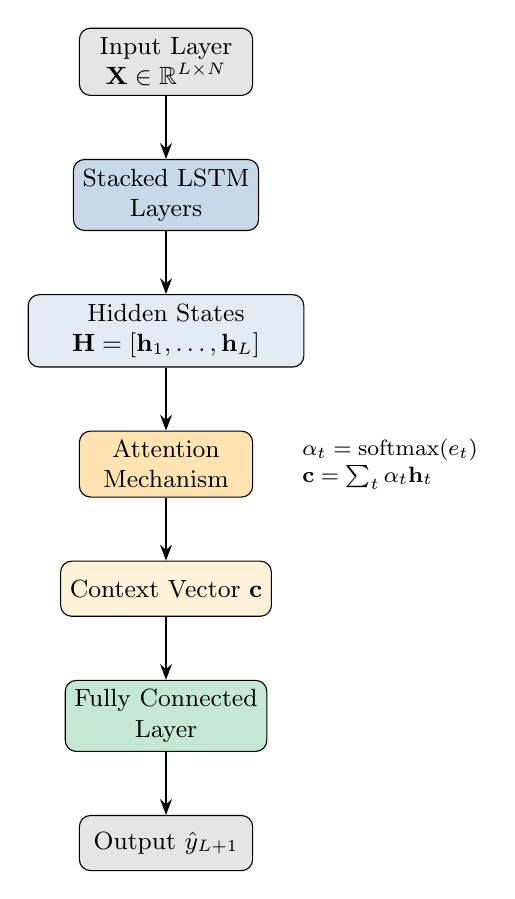
\begin{tikzpicture}[
        node distance=0.8cm,
        box/.style={rectangle, draw, rounded corners, minimum width=2.2cm, minimum height=0.7cm, align=center, font=\small},
        arrow/.style={-{Stealth[length=2mm]}, thick}
    ]
        % Input Layer
        \node[box, fill=gray!20] (input) {Input Layer\\$\mathbf{X} \in \mathbb{R}^{L \times N}$};
        
        % LSTM Layers
        \node[box, fill=lstmColor!30, below=of input] (lstm) {Stacked LSTM\\Layers};
        
        % Hidden States
        \node[box, fill=lstmColor!15, below=of lstm, minimum width=3.5cm] (hidden) {Hidden States\\$\mathbf{H} = [\mathbf{h}_1, \ldots, \mathbf{h}_L]$};
        
        % Attention
        \node[box, fill=attentionColor!30, below=of hidden] (attention) {Attention\\Mechanism};
        
        % Context Vector
        \node[box, fill=attentionColor!15, below=of attention] (context) {Context Vector $\mathbf{c}$};
        
        % FC Layer
        \node[box, fill=fcColor!30, below=of context] (fc) {Fully Connected\\Layer};
        
        % Output
        \node[box, fill=gray!20, below=of fc] (output) {Output $\hat{y}_{L+1}$};
        
        % Arrows
        \draw[arrow] (input) -- (lstm);
        \draw[arrow] (lstm) -- (hidden);
        \draw[arrow] (hidden) -- (attention);
        \draw[arrow] (attention) -- (context);
        \draw[arrow] (context) -- (fc);
        \draw[arrow] (fc) -- (output);
        
        % Side annotation
        \node[right=0.5cm of attention, align=left, font=\footnotesize] {$\alpha_t = \text{softmax}(e_t)$\\$\mathbf{c} = \sum_t \alpha_t \mathbf{h}_t$};
    \end{tikzpicture}
    \caption{Architecture of the proposed LSTM-Attention model for steering torque prediction.}
    \label{fig:architecture}
\end{figure}

\subsection{Attention Mechanisms}

To enhance the model's ability to focus on relevant time steps, we integrate attention mechanisms between the LSTM layers and the fully connected layer.
We investigate three attention mechanisms with different computational approaches.

\subsubsection{Simple Attention}

The Simple Attention mechanism independently evaluates the importance of each time step using a single linear transformation:
\begin{align}
    e_t &= \mathbf{W}_e \mathbf{h}_t + b_e \label{eq:linear_score}\\
    \alpha_t &= \frac{\exp(e_t)}{\sum_{k=1}^{L} \exp(e_k)} \label{eq:linear_weight}\\
    \mathbf{c} &= \sum_{t=1}^{L} \alpha_t \mathbf{h}_t \label{eq:linear_context}
\end{align}
where $\mathbf{W}_e \in \mathbb{R}^{1 \times d_h}$ and $b_e \in \mathbb{R}$ are learnable parameters, $d_h$ is the hidden state dimension, $\alpha_t$ are the attention weights, and $\mathbf{c}$ is the context vector.

This mechanism introduces minimal additional parameters ($d_h + 1$) while enabling the model to weight different time steps according to their relevance for prediction.

\subsubsection{Additive Attention (Bahdanau)}

Additive Attention, proposed by Bahdanau et al.~\cite{bahdanau2016neural}, computes pairwise attention scores using a feed-forward network:
\begin{align}
    e_{ij} &= \mathbf{v}_a^T \tanh(\mathbf{W}_a \mathbf{h}_i + \mathbf{U}_a \mathbf{h}_j) \label{eq:additive_score}\\
    \alpha_{ij} &= \frac{\exp(e_{ij})}{\sum_{k=1}^{L} \exp(e_{ik})} \label{eq:additive_weight}\\
    \mathbf{c}_i &= \sum_{j=1}^{L} \alpha_{ij} \mathbf{h}_j \label{eq:additive_context}
\end{align}
where $\mathbf{W}_a, \mathbf{U}_a \in \mathbb{R}^{d_a \times d_h}$ and $\mathbf{v}_a \in \mathbb{R}^{d_a}$ are learnable parameters, and $d_a$ is the attention dimension.

This mechanism captures correlations between different time steps, allowing each position to incorporate information from all other positions.
The total number of parameters is $2d_h d_a + d_a$.

\subsubsection{Scaled Dot-Product Attention (Luong)}

Scaled Dot-Product Attention computes attention scores through dot products between hidden states~\cite{vaswani2017attention}:
\begin{align}
    e_{ij} &= \frac{\mathbf{h}_i^T \mathbf{h}_j}{\sqrt{d_h}} \label{eq:dotprod_score}\\
    \alpha_{ij} &= \frac{\exp(e_{ij})}{\sum_{k=1}^{L} \exp(e_{ik})} \label{eq:dotprod_weight}\\
    \mathbf{c}_i &= \sum_{j=1}^{L} \alpha_{ij} \mathbf{h}_j \label{eq:dotprod_context}
\end{align}

The scaling factor $\sqrt{d_h}$ prevents the dot products from becoming too large for high-dimensional vectors, which would push the softmax function into regions with extremely small gradients~\cite{vaswani2017attention}.
This mechanism introduces no additional learnable parameters.

%%% Figure: Attention Mechanisms Comparison
\begin{figure}[t]
    \centering
    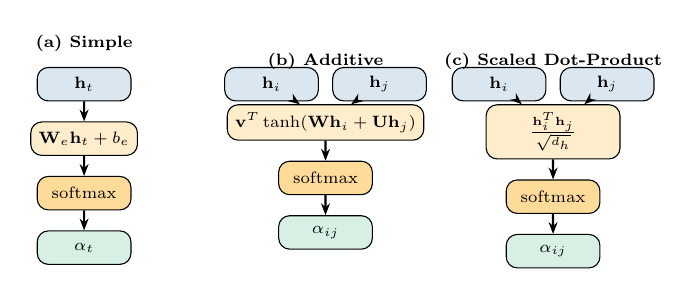
\begin{tikzpicture}[
        node distance=0.4cm,
        smallbox/.style={rectangle, draw, rounded corners, minimum width=1.4cm, minimum height=0.5cm, align=center, font=\scriptsize},
        arrow/.style={-{Stealth[length=1.5mm]}, thick},
        scale=0.85, transform shape
    ]
        % Simple Attention
        \begin{scope}[local bounding box=linear]
            \node[smallbox, fill=lstmColor!20] (h1) {$\mathbf{h}_t$};
            \node[smallbox, fill=attentionColor!20, below=0.3cm of h1] (linear) {$\mathbf{W}_e \mathbf{h}_t + b_e$};
            \node[smallbox, fill=attentionColor!40, below=0.3cm of linear] (soft1) {softmax};
            \node[smallbox, fill=fcColor!20, below=0.3cm of soft1] (alpha1) {$\alpha_t$};
            \draw[arrow] (h1) -- (linear);
            \draw[arrow] (linear) -- (soft1);
            \draw[arrow] (soft1) -- (alpha1);
            \node[above=0.1cm of h1, font=\scriptsize\bfseries] {(a) Simple};
        \end{scope}
        
        % Additive Attention
        \begin{scope}[xshift=2.8cm, local bounding box=additive]
            \node[smallbox, fill=lstmColor!20] (h2i) {$\mathbf{h}_i$};
            \node[smallbox, fill=lstmColor!20, right=0.2cm of h2i] (h2j) {$\mathbf{h}_j$};
            \node[smallbox, fill=attentionColor!20, below=0.3cm of $(h2i)!0.5!(h2j)$, minimum width=2.2cm] (add) {$\mathbf{v}^T \tanh(\mathbf{W}\mathbf{h}_i + \mathbf{U}\mathbf{h}_j)$};
            \node[smallbox, fill=attentionColor!40, below=0.3cm of add] (soft2) {softmax};
            \node[smallbox, fill=fcColor!20, below=0.3cm of soft2] (alpha2) {$\alpha_{ij}$};
            \draw[arrow] (h2i) -- (add);
            \draw[arrow] (h2j) -- (add);
            \draw[arrow] (add) -- (soft2);
            \draw[arrow] (soft2) -- (alpha2);
            \node[above=0.1cm of $(h2i)!0.5!(h2j)$, font=\scriptsize\bfseries] {(b) Additive};
        \end{scope}
        
        % Scaled Dot-Product Attention
        \begin{scope}[xshift=6.2cm, local bounding box=dotprod]
            \node[smallbox, fill=lstmColor!20] (h3i) {$\mathbf{h}_i$};
            \node[smallbox, fill=lstmColor!20, right=0.2cm of h3i] (h3j) {$\mathbf{h}_j$};
            \node[smallbox, fill=attentionColor!20, below=0.3cm of $(h3i)!0.5!(h3j)$, minimum width=2cm] (dot) {$\frac{\mathbf{h}_i^T \mathbf{h}_j}{\sqrt{d_h}}$};
            \node[smallbox, fill=attentionColor!40, below=0.3cm of dot] (soft3) {softmax};
            \node[smallbox, fill=fcColor!20, below=0.3cm of soft3] (alpha3) {$\alpha_{ij}$};
            \draw[arrow] (h3i) -- (dot);
            \draw[arrow] (h3j) -- (dot);
            \draw[arrow] (dot) -- (soft3);
            \draw[arrow] (soft3) -- (alpha3);
            \node[above=0.1cm of $(h3i)!0.5!(h3j)$, font=\scriptsize\bfseries] {(c) Scaled Dot-Product};
        \end{scope}
    \end{tikzpicture}
    \caption{Comparison of the three investigated attention mechanisms: (a) Simple Attention evaluates each time step independently, (b) Additive Attention uses a feed-forward network, and (c) Scaled Dot-Product Attention computes dot products.}
    \label{fig:attention_mechanisms}
\end{figure}

%%%
% EXPERIMENTAL SETUP
%%%
\section{Experimental Setup}
\label{sec:experimental_setup}

\subsection{Dataset}

We use the commaSteeringControl dataset~\cite{commasteeringcontrol}, which contains vehicle steering measurements collected with the openpilot ADAS system~\cite{openpilot}.
The dataset includes sensor data from various vehicle models; for this study, we select data from the 2020 Hyundai Sonata equipped with a Column-type Electric Power Steering (C-EPS) system.

Due to time and computational resource limitations, data from the first 5001 CSV files of the 2020 Hyundai Sonata were selected, each containing approximately 60 seconds of driving data recorded at 10~Hz sampling frequency.
We filter the data to include only segments where the openpilot system is fully engaged (latActive = True) and the driver is not intervening (steeringPressed = False), ensuring consistent autonomous steering behavior.

The target variable is the normalized, rate-limited steering torque (steerFiltered), ranging from $-1$ to $1$.
This normalization enables generalization across different vehicle models with varying torque ranges.

\subsection{Data Preprocessing}

Data preprocessing involves the following steps:
\begin{enumerate}
    \item Each CSV file is assigned a unique sequence ID to maintain temporal continuity.
    \item Missing and duplicate values are removed.
    \item Features are selected based on vehicle dynamics equations (\cref{eq:torque}).
    \item A sliding window technique with window size $L=50$ (5 seconds at 10~Hz) is applied to create training samples.
\end{enumerate}

The sliding window moves forward by one time step for each sample, creating overlapping sequences that capture the temporal evolution of vehicle dynamics.

\subsection{Implementation Details}

All models are implemented using the PyTorch Lightning framework (version 2.5.0) and trained on an NVIDIA GeForce RTX 2060 Super GPU with 8~GB VRAM.

The dataset is split into training (\qty{70}{\percent}), validation (\qty{20}{\percent}), and test (\qty{10}{\percent}) sets.
Training samples are shuffled to improve generalization, while validation and test samples maintain temporal order.

We use Mean Squared Error (MSE) as the loss function:
\begin{equation}
    \mathcal{L}_{\text{MSE}} = \frac{1}{n}\sum_{i=1}^{n}(y_i - \hat{y}_i)^2
    \label{eq:mse}
\end{equation}

The Adam optimizer~\cite{kingma2015adam} is used with a learning rate determined through Bayesian hyperparameter optimization using the Optuna library~\cite{akiba2019optuna} with Tree-structured Parzen Estimator (TPE).
Early stopping with patience of 5 epochs prevents overfitting.

\subsection{Evaluation Metrics}

We evaluate model performance using the following metrics:

\textbf{Accuracy:} The percentage of predictions with absolute error below a threshold $\epsilon = 0.05$:
\begin{equation}
    \text{Accuracy} = \frac{1}{n}\sum_{i=1}^{n}\mathbb{I}(|y_i - \hat{y}_i| \leq \epsilon)
    \label{eq:accuracy}
\end{equation}

\textbf{Root Mean Squared Error (RMSE):}
\begin{equation}
    \text{RMSE} = \sqrt{\frac{1}{n}\sum_{i=1}^{n}(y_i - \hat{y}_i)^2}
    \label{eq:rmse}
\end{equation}

\textbf{Inference Time:} The 95th percentile of single-sample prediction time on CPU, ensuring consistent real-time performance:
\begin{equation}
    T_{\text{inf}} = P_{95}(t_1, t_2, \ldots, t_n)
    \label{eq:inference}
\end{equation}

\textbf{Parameter Efficiency (PE):} The ratio of prediction accuracy to model size, measuring how effectively parameters are utilized:
\begin{equation}
    \text{PE} = \frac{\text{Accuracy}}{|\theta| / 10^5}
    \label{eq:param_efficiency}
\end{equation}
where $|\theta|$ denotes the total number of trainable parameters. Higher PE indicates better utilization of model capacity.

\subsection{Model Configurations}

We evaluate six model configurations combining two LSTM sizes with four attention variants, as summarized in \cref{tab:models}.

\begin{table}[t]
    \centering
    \caption{Overview of Model Configurations}
    \label{tab:models}
    \begin{tabular}{clcc}
        \toprule
        \textbf{ID} & \textbf{Description} & \textbf{Params (total)} & \textbf{Params (Attn)} \\
        \midrule
        M1 & Small Baseline & 85K & -- \\
        M2 & Small + Simple Attn & 85K & 65 \\
        \midrule
        M3 & Medium Baseline & 598K & -- \\
        M4 & Medium + Simple Attn & 598K & 129 \\
        M5 & Medium + Additive Attn & 631K & 33K \\
        M6 & Medium + Scaled DP Attn & 598K & 0 \\
        \bottomrule
    \end{tabular}
\end{table}

The small configuration uses hidden size 64 with 3 LSTM layers, while the medium configuration uses hidden size 128 with 5 layers.

%%%
% RESULTS AND DISCUSSION
%%%
\section{Results and Discussion}
\label{sec:results}

\subsection{Baseline LSTM Performance}

The small baseline LSTM model (M1) with hidden size 64 and 3 layers achieves \qty{82.57}{\percent} accuracy and RMSE of 0.0408 on the test set.
The validation accuracy increases rapidly during early training and gradually converges.

Increasing model complexity to the medium configuration (M3, hidden size 128, 5 layers) improves accuracy to \qty{87.84}{\percent}, with a 7-fold increase in model parameters (from 85K to 598K).
This improvement motivates the integration of attention mechanisms to further enhance prediction accuracy.

\subsection{Impact of Attention Mechanisms}

\cref{tab:attention_comparison} presents the performance comparison of LSTM models with different attention mechanisms.

%%% Table: Attention Comparison
\begin{table}[t]
    \centering
    \caption{Performance Comparison of LSTM Models with Different Attention Mechanisms}
    \label{tab:attention_comparison}
    \begin{tabular}{lccccc}
        \toprule
        \textbf{Model} & \textbf{Params} & \textbf{FLOPs} & \textbf{Acc. (\%)} & \textbf{RMSE} & \textbf{Inf. (ms)} \\
        \midrule
        M1 & 85K & 4.3M & 82.57 & 0.0408 & 0.92 \\
        M2 & 85K & 4.3M & 81.50 & 0.0423 & 0.97 \\
        \midrule
        M3 & 598K & 30.1M & 87.84 & 0.0338 & 2.66 \\
        \textbf{M4} & 598K & 30.1M & \textbf{90.25} & \textbf{0.0311} & 2.75 \\
        M5 & 631K & 31.8M & 88.34 & 0.0332 & 3.82 \\
        M6 & 598K & 30.1M & 88.17 & 0.0334 & 2.77 \\
        \bottomrule
    \end{tabular}
\end{table}

The medium LSTM with Simple Attention (M4) achieves the highest accuracy (\qty{90.25}{\percent}) and lowest RMSE (0.0311). Notably, attention mechanisms do not improve performance for small models: M2 (\qty{81.50}{\percent}) underperforms the baseline M1 (\qty{82.57}{\percent}), suggesting that small architectures lack sufficient representational capacity to benefit from attention weighting.

This result suggests that for steering torque prediction with medium-sized models, independently evaluating the importance of each time step is more effective than modeling complex inter-time-step dependencies.
The steering torque at a given moment is primarily influenced by recent vehicle dynamics rather than long-range correlations.

\subsection{Inference Efficiency Analysis}

For deployment in automotive embedded systems, inference time is critical. \cref{tab:inference} summarizes the computational efficiency of all models.

\begin{table}[t]
    \centering
    \caption{Inference Efficiency on Desktop CPU (AMD Ryzen 7 3700X, single-thread)}
    \label{tab:inference}
    \begin{tabular}{lccc}
        \toprule
        \textbf{Model} & \textbf{FLOPs} & \textbf{Inf. (ms)} & \textbf{Attn. Overhead} \\
        \midrule
        M1 & 4.3M & 0.92 & -- \\
        M2 & 4.3M & 0.97 & +5.4\% \\
        \midrule
        M3 & 30.1M & 2.66 & -- \\
        M4 & 30.1M & 2.75 & +3.4\% \\
        M5 & 31.8M & 3.82 & +43.6\% \\
        M6 & 30.1M & 2.77 & +4.1\% \\
        \bottomrule
    \end{tabular}
\end{table}

The computational overhead of attention mechanisms varies significantly: Simple Attention adds only \qty{3.4}{\percent} latency while providing the largest accuracy gain (\qty{+2.41}{\percent}), whereas Additive Attention increases latency by \qty{44}{\percent} for a smaller accuracy improvement (\qty{+0.50}{\percent}). This demonstrates that more complex attention mechanisms do not necessarily yield better accuracy-efficiency trade-offs for this task.

While these measurements were obtained on a desktop CPU, the computational requirements can be extrapolated to embedded platforms based on FLOPs. The small model configuration (M1, 4.3M FLOPs) requires approximately $7\times$ fewer operations than medium models, suggesting feasibility for deployment on mid-tier embedded processors such as ARM Cortex-A class devices. For highly resource-constrained automotive ECUs, model quantization or architectural optimizations would likely be required to meet strict real-time constraints below \qty{10}{\milli\second}.

\cref{fig:inference_tradeoff} visualizes the accuracy-latency trade-off across all models.

%%% Figure: Accuracy vs Inference Time (generated by scripts/generate_paper_figures.py)
\begin{figure}[t]
    \centering
    \resizebox{\columnwidth}{!}{%% Creator: Matplotlib, PGF backend
%%
%% To include the figure in your LaTeX document, write
%%   \input{<filename>.pgf}
%%
%% Make sure the required packages are loaded in your preamble
%%   \usepackage{pgf}
%%
%% Also ensure that all the required font packages are loaded; for instance,
%% the lmodern package is sometimes necessary when using math font.
%%   \usepackage{lmodern}
%%
%% Figures using additional raster images can only be included by \input if
%% they are in the same directory as the main LaTeX file. For loading figures
%% from other directories you can use the `import` package
%%   \usepackage{import}
%%
%% and then include the figures with
%%   \import{<path to file>}{<filename>.pgf}
%%
%% Matplotlib used the following preamble
%%   \def\mathdefault#1{#1}
%%   \everymath=\expandafter{\the\everymath\displaystyle}
%%   \IfFileExists{scrextend.sty}{
%%     \usepackage[fontsize=8.000000pt]{scrextend}
%%   }{
%%     \renewcommand{\normalsize}{\fontsize{8.000000}{9.600000}\selectfont}
%%     \normalsize
%%   }
%%   \usepackage{siunitx}
%%   \usepackage{amsmath}
%%   \makeatletter\@ifpackageloaded{underscore}{}{\usepackage[strings]{underscore}}\makeatother
%%
\begingroup%
\makeatletter%
\begin{pgfpicture}%
\pgfpathrectangle{\pgfpointorigin}{\pgfqpoint{3.058504in}{2.280455in}}%
\pgfusepath{use as bounding box, clip}%
\begin{pgfscope}%
\pgfsetbuttcap%
\pgfsetmiterjoin%
\definecolor{currentfill}{rgb}{1.000000,1.000000,1.000000}%
\pgfsetfillcolor{currentfill}%
\pgfsetlinewidth{0.000000pt}%
\definecolor{currentstroke}{rgb}{1.000000,1.000000,1.000000}%
\pgfsetstrokecolor{currentstroke}%
\pgfsetdash{}{0pt}%
\pgfpathmoveto{\pgfqpoint{0.000000in}{0.000000in}}%
\pgfpathlineto{\pgfqpoint{3.058504in}{0.000000in}}%
\pgfpathlineto{\pgfqpoint{3.058504in}{2.280455in}}%
\pgfpathlineto{\pgfqpoint{0.000000in}{2.280455in}}%
\pgfpathlineto{\pgfqpoint{0.000000in}{0.000000in}}%
\pgfpathclose%
\pgfusepath{fill}%
\end{pgfscope}%
\begin{pgfscope}%
\pgfsetbuttcap%
\pgfsetmiterjoin%
\definecolor{currentfill}{rgb}{1.000000,1.000000,1.000000}%
\pgfsetfillcolor{currentfill}%
\pgfsetlinewidth{0.000000pt}%
\definecolor{currentstroke}{rgb}{0.000000,0.000000,0.000000}%
\pgfsetstrokecolor{currentstroke}%
\pgfsetstrokeopacity{0.000000}%
\pgfsetdash{}{0pt}%
\pgfpathmoveto{\pgfqpoint{0.336004in}{0.311697in}}%
\pgfpathlineto{\pgfqpoint{3.048504in}{0.311697in}}%
\pgfpathlineto{\pgfqpoint{3.048504in}{2.236697in}}%
\pgfpathlineto{\pgfqpoint{0.336004in}{2.236697in}}%
\pgfpathlineto{\pgfqpoint{0.336004in}{0.311697in}}%
\pgfpathclose%
\pgfusepath{fill}%
\end{pgfscope}%
\begin{pgfscope}%
\pgfpathrectangle{\pgfqpoint{0.336004in}{0.311697in}}{\pgfqpoint{2.712500in}{1.925000in}}%
\pgfusepath{clip}%
\pgfsetbuttcap%
\pgfsetroundjoin%
\pgfsetlinewidth{0.501875pt}%
\definecolor{currentstroke}{rgb}{0.690196,0.690196,0.690196}%
\pgfsetstrokecolor{currentstroke}%
\pgfsetstrokeopacity{0.300000}%
\pgfsetdash{{1.850000pt}{0.800000pt}}{0.000000pt}%
\pgfpathmoveto{\pgfqpoint{0.562045in}{0.311697in}}%
\pgfpathlineto{\pgfqpoint{0.562045in}{2.236697in}}%
\pgfusepath{stroke}%
\end{pgfscope}%
\begin{pgfscope}%
\pgfsetbuttcap%
\pgfsetroundjoin%
\definecolor{currentfill}{rgb}{0.000000,0.000000,0.000000}%
\pgfsetfillcolor{currentfill}%
\pgfsetlinewidth{0.501875pt}%
\definecolor{currentstroke}{rgb}{0.000000,0.000000,0.000000}%
\pgfsetstrokecolor{currentstroke}%
\pgfsetdash{}{0pt}%
\pgfsys@defobject{currentmarker}{\pgfqpoint{0.000000in}{0.000000in}}{\pgfqpoint{0.000000in}{0.048611in}}{%
\pgfpathmoveto{\pgfqpoint{0.000000in}{0.000000in}}%
\pgfpathlineto{\pgfqpoint{0.000000in}{0.048611in}}%
\pgfusepath{stroke,fill}%
}%
\begin{pgfscope}%
\pgfsys@transformshift{0.562045in}{0.311697in}%
\pgfsys@useobject{currentmarker}{}%
\end{pgfscope}%
\end{pgfscope}%
\begin{pgfscope}%
\definecolor{textcolor}{rgb}{0.000000,0.000000,0.000000}%
\pgfsetstrokecolor{textcolor}%
\pgfsetfillcolor{textcolor}%
\pgftext[x=0.562045in,y=0.263086in,,top]{\color{textcolor}{\sffamily\fontsize{7.000000}{8.400000}\selectfont\catcode`\^=\active\def^{\ifmmode\sp\else\^{}\fi}\catcode`\%=\active\def%{\%}$\mathdefault{1.0}$}}%
\end{pgfscope}%
\begin{pgfscope}%
\pgfpathrectangle{\pgfqpoint{0.336004in}{0.311697in}}{\pgfqpoint{2.712500in}{1.925000in}}%
\pgfusepath{clip}%
\pgfsetbuttcap%
\pgfsetroundjoin%
\pgfsetlinewidth{0.501875pt}%
\definecolor{currentstroke}{rgb}{0.690196,0.690196,0.690196}%
\pgfsetstrokecolor{currentstroke}%
\pgfsetstrokeopacity{0.300000}%
\pgfsetdash{{1.850000pt}{0.800000pt}}{0.000000pt}%
\pgfpathmoveto{\pgfqpoint{1.127149in}{0.311697in}}%
\pgfpathlineto{\pgfqpoint{1.127149in}{2.236697in}}%
\pgfusepath{stroke}%
\end{pgfscope}%
\begin{pgfscope}%
\pgfsetbuttcap%
\pgfsetroundjoin%
\definecolor{currentfill}{rgb}{0.000000,0.000000,0.000000}%
\pgfsetfillcolor{currentfill}%
\pgfsetlinewidth{0.501875pt}%
\definecolor{currentstroke}{rgb}{0.000000,0.000000,0.000000}%
\pgfsetstrokecolor{currentstroke}%
\pgfsetdash{}{0pt}%
\pgfsys@defobject{currentmarker}{\pgfqpoint{0.000000in}{0.000000in}}{\pgfqpoint{0.000000in}{0.048611in}}{%
\pgfpathmoveto{\pgfqpoint{0.000000in}{0.000000in}}%
\pgfpathlineto{\pgfqpoint{0.000000in}{0.048611in}}%
\pgfusepath{stroke,fill}%
}%
\begin{pgfscope}%
\pgfsys@transformshift{1.127149in}{0.311697in}%
\pgfsys@useobject{currentmarker}{}%
\end{pgfscope}%
\end{pgfscope}%
\begin{pgfscope}%
\definecolor{textcolor}{rgb}{0.000000,0.000000,0.000000}%
\pgfsetstrokecolor{textcolor}%
\pgfsetfillcolor{textcolor}%
\pgftext[x=1.127149in,y=0.263086in,,top]{\color{textcolor}{\sffamily\fontsize{7.000000}{8.400000}\selectfont\catcode`\^=\active\def^{\ifmmode\sp\else\^{}\fi}\catcode`\%=\active\def%{\%}$\mathdefault{1.5}$}}%
\end{pgfscope}%
\begin{pgfscope}%
\pgfpathrectangle{\pgfqpoint{0.336004in}{0.311697in}}{\pgfqpoint{2.712500in}{1.925000in}}%
\pgfusepath{clip}%
\pgfsetbuttcap%
\pgfsetroundjoin%
\pgfsetlinewidth{0.501875pt}%
\definecolor{currentstroke}{rgb}{0.690196,0.690196,0.690196}%
\pgfsetstrokecolor{currentstroke}%
\pgfsetstrokeopacity{0.300000}%
\pgfsetdash{{1.850000pt}{0.800000pt}}{0.000000pt}%
\pgfpathmoveto{\pgfqpoint{1.692254in}{0.311697in}}%
\pgfpathlineto{\pgfqpoint{1.692254in}{2.236697in}}%
\pgfusepath{stroke}%
\end{pgfscope}%
\begin{pgfscope}%
\pgfsetbuttcap%
\pgfsetroundjoin%
\definecolor{currentfill}{rgb}{0.000000,0.000000,0.000000}%
\pgfsetfillcolor{currentfill}%
\pgfsetlinewidth{0.501875pt}%
\definecolor{currentstroke}{rgb}{0.000000,0.000000,0.000000}%
\pgfsetstrokecolor{currentstroke}%
\pgfsetdash{}{0pt}%
\pgfsys@defobject{currentmarker}{\pgfqpoint{0.000000in}{0.000000in}}{\pgfqpoint{0.000000in}{0.048611in}}{%
\pgfpathmoveto{\pgfqpoint{0.000000in}{0.000000in}}%
\pgfpathlineto{\pgfqpoint{0.000000in}{0.048611in}}%
\pgfusepath{stroke,fill}%
}%
\begin{pgfscope}%
\pgfsys@transformshift{1.692254in}{0.311697in}%
\pgfsys@useobject{currentmarker}{}%
\end{pgfscope}%
\end{pgfscope}%
\begin{pgfscope}%
\definecolor{textcolor}{rgb}{0.000000,0.000000,0.000000}%
\pgfsetstrokecolor{textcolor}%
\pgfsetfillcolor{textcolor}%
\pgftext[x=1.692254in,y=0.263086in,,top]{\color{textcolor}{\sffamily\fontsize{7.000000}{8.400000}\selectfont\catcode`\^=\active\def^{\ifmmode\sp\else\^{}\fi}\catcode`\%=\active\def%{\%}$\mathdefault{2.0}$}}%
\end{pgfscope}%
\begin{pgfscope}%
\pgfpathrectangle{\pgfqpoint{0.336004in}{0.311697in}}{\pgfqpoint{2.712500in}{1.925000in}}%
\pgfusepath{clip}%
\pgfsetbuttcap%
\pgfsetroundjoin%
\pgfsetlinewidth{0.501875pt}%
\definecolor{currentstroke}{rgb}{0.690196,0.690196,0.690196}%
\pgfsetstrokecolor{currentstroke}%
\pgfsetstrokeopacity{0.300000}%
\pgfsetdash{{1.850000pt}{0.800000pt}}{0.000000pt}%
\pgfpathmoveto{\pgfqpoint{2.257358in}{0.311697in}}%
\pgfpathlineto{\pgfqpoint{2.257358in}{2.236697in}}%
\pgfusepath{stroke}%
\end{pgfscope}%
\begin{pgfscope}%
\pgfsetbuttcap%
\pgfsetroundjoin%
\definecolor{currentfill}{rgb}{0.000000,0.000000,0.000000}%
\pgfsetfillcolor{currentfill}%
\pgfsetlinewidth{0.501875pt}%
\definecolor{currentstroke}{rgb}{0.000000,0.000000,0.000000}%
\pgfsetstrokecolor{currentstroke}%
\pgfsetdash{}{0pt}%
\pgfsys@defobject{currentmarker}{\pgfqpoint{0.000000in}{0.000000in}}{\pgfqpoint{0.000000in}{0.048611in}}{%
\pgfpathmoveto{\pgfqpoint{0.000000in}{0.000000in}}%
\pgfpathlineto{\pgfqpoint{0.000000in}{0.048611in}}%
\pgfusepath{stroke,fill}%
}%
\begin{pgfscope}%
\pgfsys@transformshift{2.257358in}{0.311697in}%
\pgfsys@useobject{currentmarker}{}%
\end{pgfscope}%
\end{pgfscope}%
\begin{pgfscope}%
\definecolor{textcolor}{rgb}{0.000000,0.000000,0.000000}%
\pgfsetstrokecolor{textcolor}%
\pgfsetfillcolor{textcolor}%
\pgftext[x=2.257358in,y=0.263086in,,top]{\color{textcolor}{\sffamily\fontsize{7.000000}{8.400000}\selectfont\catcode`\^=\active\def^{\ifmmode\sp\else\^{}\fi}\catcode`\%=\active\def%{\%}$\mathdefault{2.5}$}}%
\end{pgfscope}%
\begin{pgfscope}%
\pgfpathrectangle{\pgfqpoint{0.336004in}{0.311697in}}{\pgfqpoint{2.712500in}{1.925000in}}%
\pgfusepath{clip}%
\pgfsetbuttcap%
\pgfsetroundjoin%
\pgfsetlinewidth{0.501875pt}%
\definecolor{currentstroke}{rgb}{0.690196,0.690196,0.690196}%
\pgfsetstrokecolor{currentstroke}%
\pgfsetstrokeopacity{0.300000}%
\pgfsetdash{{1.850000pt}{0.800000pt}}{0.000000pt}%
\pgfpathmoveto{\pgfqpoint{2.822462in}{0.311697in}}%
\pgfpathlineto{\pgfqpoint{2.822462in}{2.236697in}}%
\pgfusepath{stroke}%
\end{pgfscope}%
\begin{pgfscope}%
\pgfsetbuttcap%
\pgfsetroundjoin%
\definecolor{currentfill}{rgb}{0.000000,0.000000,0.000000}%
\pgfsetfillcolor{currentfill}%
\pgfsetlinewidth{0.501875pt}%
\definecolor{currentstroke}{rgb}{0.000000,0.000000,0.000000}%
\pgfsetstrokecolor{currentstroke}%
\pgfsetdash{}{0pt}%
\pgfsys@defobject{currentmarker}{\pgfqpoint{0.000000in}{0.000000in}}{\pgfqpoint{0.000000in}{0.048611in}}{%
\pgfpathmoveto{\pgfqpoint{0.000000in}{0.000000in}}%
\pgfpathlineto{\pgfqpoint{0.000000in}{0.048611in}}%
\pgfusepath{stroke,fill}%
}%
\begin{pgfscope}%
\pgfsys@transformshift{2.822462in}{0.311697in}%
\pgfsys@useobject{currentmarker}{}%
\end{pgfscope}%
\end{pgfscope}%
\begin{pgfscope}%
\definecolor{textcolor}{rgb}{0.000000,0.000000,0.000000}%
\pgfsetstrokecolor{textcolor}%
\pgfsetfillcolor{textcolor}%
\pgftext[x=2.822462in,y=0.263086in,,top]{\color{textcolor}{\sffamily\fontsize{7.000000}{8.400000}\selectfont\catcode`\^=\active\def^{\ifmmode\sp\else\^{}\fi}\catcode`\%=\active\def%{\%}$\mathdefault{3.0}$}}%
\end{pgfscope}%
\begin{pgfscope}%
\definecolor{textcolor}{rgb}{0.000000,0.000000,0.000000}%
\pgfsetstrokecolor{textcolor}%
\pgfsetfillcolor{textcolor}%
\pgftext[x=1.692254in,y=0.121111in,,top]{\color{textcolor}{\sffamily\fontsize{8.000000}{9.600000}\selectfont\catcode`\^=\active\def^{\ifmmode\sp\else\^{}\fi}\catcode`\%=\active\def%{\%}Inference Time P95 (ms)}}%
\end{pgfscope}%
\begin{pgfscope}%
\pgfpathrectangle{\pgfqpoint{0.336004in}{0.311697in}}{\pgfqpoint{2.712500in}{1.925000in}}%
\pgfusepath{clip}%
\pgfsetbuttcap%
\pgfsetroundjoin%
\pgfsetlinewidth{0.501875pt}%
\definecolor{currentstroke}{rgb}{0.690196,0.690196,0.690196}%
\pgfsetstrokecolor{currentstroke}%
\pgfsetstrokeopacity{0.300000}%
\pgfsetdash{{1.850000pt}{0.800000pt}}{0.000000pt}%
\pgfpathmoveto{\pgfqpoint{0.336004in}{0.311697in}}%
\pgfpathlineto{\pgfqpoint{3.048504in}{0.311697in}}%
\pgfusepath{stroke}%
\end{pgfscope}%
\begin{pgfscope}%
\pgfsetbuttcap%
\pgfsetroundjoin%
\definecolor{currentfill}{rgb}{0.000000,0.000000,0.000000}%
\pgfsetfillcolor{currentfill}%
\pgfsetlinewidth{0.501875pt}%
\definecolor{currentstroke}{rgb}{0.000000,0.000000,0.000000}%
\pgfsetstrokecolor{currentstroke}%
\pgfsetdash{}{0pt}%
\pgfsys@defobject{currentmarker}{\pgfqpoint{0.000000in}{0.000000in}}{\pgfqpoint{0.048611in}{0.000000in}}{%
\pgfpathmoveto{\pgfqpoint{0.000000in}{0.000000in}}%
\pgfpathlineto{\pgfqpoint{0.048611in}{0.000000in}}%
\pgfusepath{stroke,fill}%
}%
\begin{pgfscope}%
\pgfsys@transformshift{0.336004in}{0.311697in}%
\pgfsys@useobject{currentmarker}{}%
\end{pgfscope}%
\end{pgfscope}%
\begin{pgfscope}%
\definecolor{textcolor}{rgb}{0.000000,0.000000,0.000000}%
\pgfsetstrokecolor{textcolor}%
\pgfsetfillcolor{textcolor}%
\pgftext[x=0.176667in, y=0.277940in, left, base]{\color{textcolor}{\sffamily\fontsize{7.000000}{8.400000}\selectfont\catcode`\^=\active\def^{\ifmmode\sp\else\^{}\fi}\catcode`\%=\active\def%{\%}$\mathdefault{80}$}}%
\end{pgfscope}%
\begin{pgfscope}%
\pgfpathrectangle{\pgfqpoint{0.336004in}{0.311697in}}{\pgfqpoint{2.712500in}{1.925000in}}%
\pgfusepath{clip}%
\pgfsetbuttcap%
\pgfsetroundjoin%
\pgfsetlinewidth{0.501875pt}%
\definecolor{currentstroke}{rgb}{0.690196,0.690196,0.690196}%
\pgfsetstrokecolor{currentstroke}%
\pgfsetstrokeopacity{0.300000}%
\pgfsetdash{{1.850000pt}{0.800000pt}}{0.000000pt}%
\pgfpathmoveto{\pgfqpoint{0.336004in}{0.632531in}}%
\pgfpathlineto{\pgfqpoint{3.048504in}{0.632531in}}%
\pgfusepath{stroke}%
\end{pgfscope}%
\begin{pgfscope}%
\pgfsetbuttcap%
\pgfsetroundjoin%
\definecolor{currentfill}{rgb}{0.000000,0.000000,0.000000}%
\pgfsetfillcolor{currentfill}%
\pgfsetlinewidth{0.501875pt}%
\definecolor{currentstroke}{rgb}{0.000000,0.000000,0.000000}%
\pgfsetstrokecolor{currentstroke}%
\pgfsetdash{}{0pt}%
\pgfsys@defobject{currentmarker}{\pgfqpoint{0.000000in}{0.000000in}}{\pgfqpoint{0.048611in}{0.000000in}}{%
\pgfpathmoveto{\pgfqpoint{0.000000in}{0.000000in}}%
\pgfpathlineto{\pgfqpoint{0.048611in}{0.000000in}}%
\pgfusepath{stroke,fill}%
}%
\begin{pgfscope}%
\pgfsys@transformshift{0.336004in}{0.632531in}%
\pgfsys@useobject{currentmarker}{}%
\end{pgfscope}%
\end{pgfscope}%
\begin{pgfscope}%
\definecolor{textcolor}{rgb}{0.000000,0.000000,0.000000}%
\pgfsetstrokecolor{textcolor}%
\pgfsetfillcolor{textcolor}%
\pgftext[x=0.176667in, y=0.598773in, left, base]{\color{textcolor}{\sffamily\fontsize{7.000000}{8.400000}\selectfont\catcode`\^=\active\def^{\ifmmode\sp\else\^{}\fi}\catcode`\%=\active\def%{\%}$\mathdefault{82}$}}%
\end{pgfscope}%
\begin{pgfscope}%
\pgfpathrectangle{\pgfqpoint{0.336004in}{0.311697in}}{\pgfqpoint{2.712500in}{1.925000in}}%
\pgfusepath{clip}%
\pgfsetbuttcap%
\pgfsetroundjoin%
\pgfsetlinewidth{0.501875pt}%
\definecolor{currentstroke}{rgb}{0.690196,0.690196,0.690196}%
\pgfsetstrokecolor{currentstroke}%
\pgfsetstrokeopacity{0.300000}%
\pgfsetdash{{1.850000pt}{0.800000pt}}{0.000000pt}%
\pgfpathmoveto{\pgfqpoint{0.336004in}{0.953364in}}%
\pgfpathlineto{\pgfqpoint{3.048504in}{0.953364in}}%
\pgfusepath{stroke}%
\end{pgfscope}%
\begin{pgfscope}%
\pgfsetbuttcap%
\pgfsetroundjoin%
\definecolor{currentfill}{rgb}{0.000000,0.000000,0.000000}%
\pgfsetfillcolor{currentfill}%
\pgfsetlinewidth{0.501875pt}%
\definecolor{currentstroke}{rgb}{0.000000,0.000000,0.000000}%
\pgfsetstrokecolor{currentstroke}%
\pgfsetdash{}{0pt}%
\pgfsys@defobject{currentmarker}{\pgfqpoint{0.000000in}{0.000000in}}{\pgfqpoint{0.048611in}{0.000000in}}{%
\pgfpathmoveto{\pgfqpoint{0.000000in}{0.000000in}}%
\pgfpathlineto{\pgfqpoint{0.048611in}{0.000000in}}%
\pgfusepath{stroke,fill}%
}%
\begin{pgfscope}%
\pgfsys@transformshift{0.336004in}{0.953364in}%
\pgfsys@useobject{currentmarker}{}%
\end{pgfscope}%
\end{pgfscope}%
\begin{pgfscope}%
\definecolor{textcolor}{rgb}{0.000000,0.000000,0.000000}%
\pgfsetstrokecolor{textcolor}%
\pgfsetfillcolor{textcolor}%
\pgftext[x=0.176667in, y=0.919606in, left, base]{\color{textcolor}{\sffamily\fontsize{7.000000}{8.400000}\selectfont\catcode`\^=\active\def^{\ifmmode\sp\else\^{}\fi}\catcode`\%=\active\def%{\%}$\mathdefault{84}$}}%
\end{pgfscope}%
\begin{pgfscope}%
\pgfpathrectangle{\pgfqpoint{0.336004in}{0.311697in}}{\pgfqpoint{2.712500in}{1.925000in}}%
\pgfusepath{clip}%
\pgfsetbuttcap%
\pgfsetroundjoin%
\pgfsetlinewidth{0.501875pt}%
\definecolor{currentstroke}{rgb}{0.690196,0.690196,0.690196}%
\pgfsetstrokecolor{currentstroke}%
\pgfsetstrokeopacity{0.300000}%
\pgfsetdash{{1.850000pt}{0.800000pt}}{0.000000pt}%
\pgfpathmoveto{\pgfqpoint{0.336004in}{1.274197in}}%
\pgfpathlineto{\pgfqpoint{3.048504in}{1.274197in}}%
\pgfusepath{stroke}%
\end{pgfscope}%
\begin{pgfscope}%
\pgfsetbuttcap%
\pgfsetroundjoin%
\definecolor{currentfill}{rgb}{0.000000,0.000000,0.000000}%
\pgfsetfillcolor{currentfill}%
\pgfsetlinewidth{0.501875pt}%
\definecolor{currentstroke}{rgb}{0.000000,0.000000,0.000000}%
\pgfsetstrokecolor{currentstroke}%
\pgfsetdash{}{0pt}%
\pgfsys@defobject{currentmarker}{\pgfqpoint{0.000000in}{0.000000in}}{\pgfqpoint{0.048611in}{0.000000in}}{%
\pgfpathmoveto{\pgfqpoint{0.000000in}{0.000000in}}%
\pgfpathlineto{\pgfqpoint{0.048611in}{0.000000in}}%
\pgfusepath{stroke,fill}%
}%
\begin{pgfscope}%
\pgfsys@transformshift{0.336004in}{1.274197in}%
\pgfsys@useobject{currentmarker}{}%
\end{pgfscope}%
\end{pgfscope}%
\begin{pgfscope}%
\definecolor{textcolor}{rgb}{0.000000,0.000000,0.000000}%
\pgfsetstrokecolor{textcolor}%
\pgfsetfillcolor{textcolor}%
\pgftext[x=0.176667in, y=1.240440in, left, base]{\color{textcolor}{\sffamily\fontsize{7.000000}{8.400000}\selectfont\catcode`\^=\active\def^{\ifmmode\sp\else\^{}\fi}\catcode`\%=\active\def%{\%}$\mathdefault{86}$}}%
\end{pgfscope}%
\begin{pgfscope}%
\pgfpathrectangle{\pgfqpoint{0.336004in}{0.311697in}}{\pgfqpoint{2.712500in}{1.925000in}}%
\pgfusepath{clip}%
\pgfsetbuttcap%
\pgfsetroundjoin%
\pgfsetlinewidth{0.501875pt}%
\definecolor{currentstroke}{rgb}{0.690196,0.690196,0.690196}%
\pgfsetstrokecolor{currentstroke}%
\pgfsetstrokeopacity{0.300000}%
\pgfsetdash{{1.850000pt}{0.800000pt}}{0.000000pt}%
\pgfpathmoveto{\pgfqpoint{0.336004in}{1.595031in}}%
\pgfpathlineto{\pgfqpoint{3.048504in}{1.595031in}}%
\pgfusepath{stroke}%
\end{pgfscope}%
\begin{pgfscope}%
\pgfsetbuttcap%
\pgfsetroundjoin%
\definecolor{currentfill}{rgb}{0.000000,0.000000,0.000000}%
\pgfsetfillcolor{currentfill}%
\pgfsetlinewidth{0.501875pt}%
\definecolor{currentstroke}{rgb}{0.000000,0.000000,0.000000}%
\pgfsetstrokecolor{currentstroke}%
\pgfsetdash{}{0pt}%
\pgfsys@defobject{currentmarker}{\pgfqpoint{0.000000in}{0.000000in}}{\pgfqpoint{0.048611in}{0.000000in}}{%
\pgfpathmoveto{\pgfqpoint{0.000000in}{0.000000in}}%
\pgfpathlineto{\pgfqpoint{0.048611in}{0.000000in}}%
\pgfusepath{stroke,fill}%
}%
\begin{pgfscope}%
\pgfsys@transformshift{0.336004in}{1.595031in}%
\pgfsys@useobject{currentmarker}{}%
\end{pgfscope}%
\end{pgfscope}%
\begin{pgfscope}%
\definecolor{textcolor}{rgb}{0.000000,0.000000,0.000000}%
\pgfsetstrokecolor{textcolor}%
\pgfsetfillcolor{textcolor}%
\pgftext[x=0.176667in, y=1.561273in, left, base]{\color{textcolor}{\sffamily\fontsize{7.000000}{8.400000}\selectfont\catcode`\^=\active\def^{\ifmmode\sp\else\^{}\fi}\catcode`\%=\active\def%{\%}$\mathdefault{88}$}}%
\end{pgfscope}%
\begin{pgfscope}%
\pgfpathrectangle{\pgfqpoint{0.336004in}{0.311697in}}{\pgfqpoint{2.712500in}{1.925000in}}%
\pgfusepath{clip}%
\pgfsetbuttcap%
\pgfsetroundjoin%
\pgfsetlinewidth{0.501875pt}%
\definecolor{currentstroke}{rgb}{0.690196,0.690196,0.690196}%
\pgfsetstrokecolor{currentstroke}%
\pgfsetstrokeopacity{0.300000}%
\pgfsetdash{{1.850000pt}{0.800000pt}}{0.000000pt}%
\pgfpathmoveto{\pgfqpoint{0.336004in}{1.915864in}}%
\pgfpathlineto{\pgfqpoint{3.048504in}{1.915864in}}%
\pgfusepath{stroke}%
\end{pgfscope}%
\begin{pgfscope}%
\pgfsetbuttcap%
\pgfsetroundjoin%
\definecolor{currentfill}{rgb}{0.000000,0.000000,0.000000}%
\pgfsetfillcolor{currentfill}%
\pgfsetlinewidth{0.501875pt}%
\definecolor{currentstroke}{rgb}{0.000000,0.000000,0.000000}%
\pgfsetstrokecolor{currentstroke}%
\pgfsetdash{}{0pt}%
\pgfsys@defobject{currentmarker}{\pgfqpoint{0.000000in}{0.000000in}}{\pgfqpoint{0.048611in}{0.000000in}}{%
\pgfpathmoveto{\pgfqpoint{0.000000in}{0.000000in}}%
\pgfpathlineto{\pgfqpoint{0.048611in}{0.000000in}}%
\pgfusepath{stroke,fill}%
}%
\begin{pgfscope}%
\pgfsys@transformshift{0.336004in}{1.915864in}%
\pgfsys@useobject{currentmarker}{}%
\end{pgfscope}%
\end{pgfscope}%
\begin{pgfscope}%
\definecolor{textcolor}{rgb}{0.000000,0.000000,0.000000}%
\pgfsetstrokecolor{textcolor}%
\pgfsetfillcolor{textcolor}%
\pgftext[x=0.176667in, y=1.882106in, left, base]{\color{textcolor}{\sffamily\fontsize{7.000000}{8.400000}\selectfont\catcode`\^=\active\def^{\ifmmode\sp\else\^{}\fi}\catcode`\%=\active\def%{\%}$\mathdefault{90}$}}%
\end{pgfscope}%
\begin{pgfscope}%
\pgfpathrectangle{\pgfqpoint{0.336004in}{0.311697in}}{\pgfqpoint{2.712500in}{1.925000in}}%
\pgfusepath{clip}%
\pgfsetbuttcap%
\pgfsetroundjoin%
\pgfsetlinewidth{0.501875pt}%
\definecolor{currentstroke}{rgb}{0.690196,0.690196,0.690196}%
\pgfsetstrokecolor{currentstroke}%
\pgfsetstrokeopacity{0.300000}%
\pgfsetdash{{1.850000pt}{0.800000pt}}{0.000000pt}%
\pgfpathmoveto{\pgfqpoint{0.336004in}{2.236697in}}%
\pgfpathlineto{\pgfqpoint{3.048504in}{2.236697in}}%
\pgfusepath{stroke}%
\end{pgfscope}%
\begin{pgfscope}%
\pgfsetbuttcap%
\pgfsetroundjoin%
\definecolor{currentfill}{rgb}{0.000000,0.000000,0.000000}%
\pgfsetfillcolor{currentfill}%
\pgfsetlinewidth{0.501875pt}%
\definecolor{currentstroke}{rgb}{0.000000,0.000000,0.000000}%
\pgfsetstrokecolor{currentstroke}%
\pgfsetdash{}{0pt}%
\pgfsys@defobject{currentmarker}{\pgfqpoint{0.000000in}{0.000000in}}{\pgfqpoint{0.048611in}{0.000000in}}{%
\pgfpathmoveto{\pgfqpoint{0.000000in}{0.000000in}}%
\pgfpathlineto{\pgfqpoint{0.048611in}{0.000000in}}%
\pgfusepath{stroke,fill}%
}%
\begin{pgfscope}%
\pgfsys@transformshift{0.336004in}{2.236697in}%
\pgfsys@useobject{currentmarker}{}%
\end{pgfscope}%
\end{pgfscope}%
\begin{pgfscope}%
\definecolor{textcolor}{rgb}{0.000000,0.000000,0.000000}%
\pgfsetstrokecolor{textcolor}%
\pgfsetfillcolor{textcolor}%
\pgftext[x=0.176667in, y=2.202940in, left, base]{\color{textcolor}{\sffamily\fontsize{7.000000}{8.400000}\selectfont\catcode`\^=\active\def^{\ifmmode\sp\else\^{}\fi}\catcode`\%=\active\def%{\%}$\mathdefault{92}$}}%
\end{pgfscope}%
\begin{pgfscope}%
\definecolor{textcolor}{rgb}{0.000000,0.000000,0.000000}%
\pgfsetstrokecolor{textcolor}%
\pgfsetfillcolor{textcolor}%
\pgftext[x=0.121111in,y=1.274197in,,bottom,rotate=90.000000]{\color{textcolor}{\sffamily\fontsize{8.000000}{9.600000}\selectfont\catcode`\^=\active\def^{\ifmmode\sp\else\^{}\fi}\catcode`\%=\active\def%{\%}Accuracy (\%)}}%
\end{pgfscope}%
\begin{pgfscope}%
\pgfsetrectcap%
\pgfsetmiterjoin%
\pgfsetlinewidth{0.501875pt}%
\definecolor{currentstroke}{rgb}{0.000000,0.000000,0.000000}%
\pgfsetstrokecolor{currentstroke}%
\pgfsetdash{}{0pt}%
\pgfpathmoveto{\pgfqpoint{0.336004in}{0.311697in}}%
\pgfpathlineto{\pgfqpoint{0.336004in}{2.236697in}}%
\pgfusepath{stroke}%
\end{pgfscope}%
\begin{pgfscope}%
\pgfsetrectcap%
\pgfsetmiterjoin%
\pgfsetlinewidth{0.501875pt}%
\definecolor{currentstroke}{rgb}{0.000000,0.000000,0.000000}%
\pgfsetstrokecolor{currentstroke}%
\pgfsetdash{}{0pt}%
\pgfpathmoveto{\pgfqpoint{3.048504in}{0.311697in}}%
\pgfpathlineto{\pgfqpoint{3.048504in}{2.236697in}}%
\pgfusepath{stroke}%
\end{pgfscope}%
\begin{pgfscope}%
\pgfsetrectcap%
\pgfsetmiterjoin%
\pgfsetlinewidth{0.501875pt}%
\definecolor{currentstroke}{rgb}{0.000000,0.000000,0.000000}%
\pgfsetstrokecolor{currentstroke}%
\pgfsetdash{}{0pt}%
\pgfpathmoveto{\pgfqpoint{0.336004in}{0.311697in}}%
\pgfpathlineto{\pgfqpoint{3.048504in}{0.311697in}}%
\pgfusepath{stroke}%
\end{pgfscope}%
\begin{pgfscope}%
\pgfsetrectcap%
\pgfsetmiterjoin%
\pgfsetlinewidth{0.501875pt}%
\definecolor{currentstroke}{rgb}{0.000000,0.000000,0.000000}%
\pgfsetstrokecolor{currentstroke}%
\pgfsetdash{}{0pt}%
\pgfpathmoveto{\pgfqpoint{0.336004in}{2.236697in}}%
\pgfpathlineto{\pgfqpoint{3.048504in}{2.236697in}}%
\pgfusepath{stroke}%
\end{pgfscope}%
\begin{pgfscope}%
\pgfpathrectangle{\pgfqpoint{0.336004in}{0.311697in}}{\pgfqpoint{2.712500in}{1.925000in}}%
\pgfusepath{clip}%
\pgfsetbuttcap%
\pgfsetroundjoin%
\definecolor{currentfill}{rgb}{0.000000,0.447059,0.741176}%
\pgfsetfillcolor{currentfill}%
\pgfsetlinewidth{0.501875pt}%
\definecolor{currentstroke}{rgb}{1.000000,1.000000,1.000000}%
\pgfsetstrokecolor{currentstroke}%
\pgfsetdash{}{0pt}%
\pgfsys@defobject{currentmarker}{\pgfqpoint{-0.043921in}{-0.043921in}}{\pgfqpoint{0.043921in}{0.043921in}}{%
\pgfpathmoveto{\pgfqpoint{0.000000in}{-0.043921in}}%
\pgfpathcurveto{\pgfqpoint{0.011648in}{-0.043921in}}{\pgfqpoint{0.022820in}{-0.039293in}}{\pgfqpoint{0.031056in}{-0.031056in}}%
\pgfpathcurveto{\pgfqpoint{0.039293in}{-0.022820in}}{\pgfqpoint{0.043921in}{-0.011648in}}{\pgfqpoint{0.043921in}{0.000000in}}%
\pgfpathcurveto{\pgfqpoint{0.043921in}{0.011648in}}{\pgfqpoint{0.039293in}{0.022820in}}{\pgfqpoint{0.031056in}{0.031056in}}%
\pgfpathcurveto{\pgfqpoint{0.022820in}{0.039293in}}{\pgfqpoint{0.011648in}{0.043921in}}{\pgfqpoint{0.000000in}{0.043921in}}%
\pgfpathcurveto{\pgfqpoint{-0.011648in}{0.043921in}}{\pgfqpoint{-0.022820in}{0.039293in}}{\pgfqpoint{-0.031056in}{0.031056in}}%
\pgfpathcurveto{\pgfqpoint{-0.039293in}{0.022820in}}{\pgfqpoint{-0.043921in}{0.011648in}}{\pgfqpoint{-0.043921in}{0.000000in}}%
\pgfpathcurveto{\pgfqpoint{-0.043921in}{-0.011648in}}{\pgfqpoint{-0.039293in}{-0.022820in}}{\pgfqpoint{-0.031056in}{-0.031056in}}%
\pgfpathcurveto{\pgfqpoint{-0.022820in}{-0.039293in}}{\pgfqpoint{-0.011648in}{-0.043921in}}{\pgfqpoint{0.000000in}{-0.043921in}}%
\pgfpathlineto{\pgfqpoint{0.000000in}{-0.043921in}}%
\pgfpathclose%
\pgfusepath{stroke,fill}%
}%
\begin{pgfscope}%
\pgfsys@transformshift{0.686368in}{0.723968in}%
\pgfsys@useobject{currentmarker}{}%
\end{pgfscope}%
\begin{pgfscope}%
\pgfsys@transformshift{0.742879in}{0.552322in}%
\pgfsys@useobject{currentmarker}{}%
\end{pgfscope}%
\end{pgfscope}%
\begin{pgfscope}%
\pgfpathrectangle{\pgfqpoint{0.336004in}{0.311697in}}{\pgfqpoint{2.712500in}{1.925000in}}%
\pgfusepath{clip}%
\pgfsetbuttcap%
\pgfsetroundjoin%
\definecolor{currentfill}{rgb}{0.466667,0.674510,0.188235}%
\pgfsetfillcolor{currentfill}%
\pgfsetlinewidth{0.501875pt}%
\definecolor{currentstroke}{rgb}{1.000000,1.000000,1.000000}%
\pgfsetstrokecolor{currentstroke}%
\pgfsetdash{}{0pt}%
\pgfsys@defobject{currentmarker}{\pgfqpoint{-0.046585in}{-0.046585in}}{\pgfqpoint{0.046585in}{0.046585in}}{%
\pgfpathmoveto{\pgfqpoint{-0.046585in}{-0.046585in}}%
\pgfpathlineto{\pgfqpoint{0.046585in}{-0.046585in}}%
\pgfpathlineto{\pgfqpoint{0.046585in}{0.046585in}}%
\pgfpathlineto{\pgfqpoint{-0.046585in}{0.046585in}}%
\pgfpathlineto{\pgfqpoint{-0.046585in}{-0.046585in}}%
\pgfpathclose%
\pgfusepath{stroke,fill}%
}%
\begin{pgfscope}%
\pgfsys@transformshift{2.144337in}{1.569364in}%
\pgfsys@useobject{currentmarker}{}%
\end{pgfscope}%
\end{pgfscope}%
\begin{pgfscope}%
\pgfpathrectangle{\pgfqpoint{0.336004in}{0.311697in}}{\pgfqpoint{2.712500in}{1.925000in}}%
\pgfusepath{clip}%
\pgfsetbuttcap%
\pgfsetroundjoin%
\definecolor{currentfill}{rgb}{0.850980,0.325490,0.098039}%
\pgfsetfillcolor{currentfill}%
\pgfsetlinewidth{0.501875pt}%
\definecolor{currentstroke}{rgb}{1.000000,1.000000,1.000000}%
\pgfsetstrokecolor{currentstroke}%
\pgfsetdash{}{0pt}%
\pgfsys@defobject{currentmarker}{\pgfqpoint{-0.049105in}{-0.049105in}}{\pgfqpoint{0.049105in}{0.049105in}}{%
\pgfpathmoveto{\pgfqpoint{0.000000in}{0.049105in}}%
\pgfpathlineto{\pgfqpoint{-0.049105in}{-0.049105in}}%
\pgfpathlineto{\pgfqpoint{0.049105in}{-0.049105in}}%
\pgfpathlineto{\pgfqpoint{0.000000in}{0.049105in}}%
\pgfpathclose%
\pgfusepath{stroke,fill}%
}%
\begin{pgfscope}%
\pgfsys@transformshift{2.189545in}{1.955968in}%
\pgfsys@useobject{currentmarker}{}%
\end{pgfscope}%
\begin{pgfscope}%
\pgfsys@transformshift{2.686837in}{1.649572in}%
\pgfsys@useobject{currentmarker}{}%
\end{pgfscope}%
\begin{pgfscope}%
\pgfsys@transformshift{2.212149in}{1.622301in}%
\pgfsys@useobject{currentmarker}{}%
\end{pgfscope}%
\end{pgfscope}%
\begin{pgfscope}%
\definecolor{textcolor}{rgb}{0.000000,0.000000,0.000000}%
\pgfsetstrokecolor{textcolor}%
\pgfsetfillcolor{textcolor}%
\pgftext[x=0.755813in,y=0.765635in,left,base]{\color{textcolor}{\sffamily\fontsize{8.000000}{9.600000}\selectfont\catcode`\^=\active\def^{\ifmmode\sp\else\^{}\fi}\catcode`\%=\active\def%{\%}M1}}%
\end{pgfscope}%
\begin{pgfscope}%
\definecolor{textcolor}{rgb}{0.000000,0.000000,0.000000}%
\pgfsetstrokecolor{textcolor}%
\pgfsetfillcolor{textcolor}%
\pgftext[x=0.812323in,y=0.441211in,left,base]{\color{textcolor}{\sffamily\fontsize{8.000000}{9.600000}\selectfont\catcode`\^=\active\def^{\ifmmode\sp\else\^{}\fi}\catcode`\%=\active\def%{\%}M2}}%
\end{pgfscope}%
\begin{pgfscope}%
\definecolor{textcolor}{rgb}{0.000000,0.000000,0.000000}%
\pgfsetstrokecolor{textcolor}%
\pgfsetfillcolor{textcolor}%
\pgftext[x=2.074892in,y=1.611031in,right,base]{\color{textcolor}{\sffamily\fontsize{8.000000}{9.600000}\selectfont\catcode`\^=\active\def^{\ifmmode\sp\else\^{}\fi}\catcode`\%=\active\def%{\%}M3}}%
\end{pgfscope}%
\begin{pgfscope}%
\definecolor{textcolor}{rgb}{0.000000,0.000000,0.000000}%
\pgfsetstrokecolor{textcolor}%
\pgfsetfillcolor{textcolor}%
\pgftext[x=2.258990in,y=2.025412in,left,base]{\color{textcolor}{\sffamily\fontsize{8.000000}{9.600000}\bfseries\selectfont\catcode`\^=\active\def^{\ifmmode\sp\else\^{}\fi}\catcode`\%=\active\def%{\%}M4}}%
\end{pgfscope}%
\begin{pgfscope}%
\definecolor{textcolor}{rgb}{0.000000,0.000000,0.000000}%
\pgfsetstrokecolor{textcolor}%
\pgfsetfillcolor{textcolor}%
\pgftext[x=2.756281in,y=1.691239in,left,base]{\color{textcolor}{\sffamily\fontsize{8.000000}{9.600000}\selectfont\catcode`\^=\active\def^{\ifmmode\sp\else\^{}\fi}\catcode`\%=\active\def%{\%}M5}}%
\end{pgfscope}%
\begin{pgfscope}%
\definecolor{textcolor}{rgb}{0.000000,0.000000,0.000000}%
\pgfsetstrokecolor{textcolor}%
\pgfsetfillcolor{textcolor}%
\pgftext[x=2.281594in,y=1.511190in,left,base]{\color{textcolor}{\sffamily\fontsize{8.000000}{9.600000}\selectfont\catcode`\^=\active\def^{\ifmmode\sp\else\^{}\fi}\catcode`\%=\active\def%{\%}M6}}%
\end{pgfscope}%
\begin{pgfscope}%
\pgfsetbuttcap%
\pgfsetmiterjoin%
\definecolor{currentfill}{rgb}{1.000000,1.000000,1.000000}%
\pgfsetfillcolor{currentfill}%
\pgfsetfillopacity{0.900000}%
\pgfsetlinewidth{1.003750pt}%
\definecolor{currentstroke}{rgb}{0.800000,0.800000,0.800000}%
\pgfsetstrokecolor{currentstroke}%
\pgfsetstrokeopacity{0.900000}%
\pgfsetdash{}{0pt}%
\pgfpathmoveto{\pgfqpoint{1.591508in}{0.360308in}}%
\pgfpathlineto{\pgfqpoint{2.980448in}{0.360308in}}%
\pgfpathquadraticcurveto{\pgfqpoint{2.999893in}{0.360308in}}{\pgfqpoint{2.999893in}{0.379753in}}%
\pgfpathlineto{\pgfqpoint{2.999893in}{0.797268in}}%
\pgfpathquadraticcurveto{\pgfqpoint{2.999893in}{0.816713in}}{\pgfqpoint{2.980448in}{0.816713in}}%
\pgfpathlineto{\pgfqpoint{1.591508in}{0.816713in}}%
\pgfpathquadraticcurveto{\pgfqpoint{1.572063in}{0.816713in}}{\pgfqpoint{1.572063in}{0.797268in}}%
\pgfpathlineto{\pgfqpoint{1.572063in}{0.379753in}}%
\pgfpathquadraticcurveto{\pgfqpoint{1.572063in}{0.360308in}}{\pgfqpoint{1.591508in}{0.360308in}}%
\pgfpathlineto{\pgfqpoint{1.591508in}{0.360308in}}%
\pgfpathclose%
\pgfusepath{stroke,fill}%
\end{pgfscope}%
\begin{pgfscope}%
\pgfsetbuttcap%
\pgfsetroundjoin%
\definecolor{currentfill}{rgb}{0.000000,0.447059,0.741176}%
\pgfsetfillcolor{currentfill}%
\pgfsetlinewidth{0.501875pt}%
\definecolor{currentstroke}{rgb}{1.000000,1.000000,1.000000}%
\pgfsetstrokecolor{currentstroke}%
\pgfsetdash{}{0pt}%
\pgfsys@defobject{currentmarker}{\pgfqpoint{-0.043921in}{-0.043921in}}{\pgfqpoint{0.043921in}{0.043921in}}{%
\pgfpathmoveto{\pgfqpoint{0.000000in}{-0.043921in}}%
\pgfpathcurveto{\pgfqpoint{0.011648in}{-0.043921in}}{\pgfqpoint{0.022820in}{-0.039293in}}{\pgfqpoint{0.031056in}{-0.031056in}}%
\pgfpathcurveto{\pgfqpoint{0.039293in}{-0.022820in}}{\pgfqpoint{0.043921in}{-0.011648in}}{\pgfqpoint{0.043921in}{0.000000in}}%
\pgfpathcurveto{\pgfqpoint{0.043921in}{0.011648in}}{\pgfqpoint{0.039293in}{0.022820in}}{\pgfqpoint{0.031056in}{0.031056in}}%
\pgfpathcurveto{\pgfqpoint{0.022820in}{0.039293in}}{\pgfqpoint{0.011648in}{0.043921in}}{\pgfqpoint{0.000000in}{0.043921in}}%
\pgfpathcurveto{\pgfqpoint{-0.011648in}{0.043921in}}{\pgfqpoint{-0.022820in}{0.039293in}}{\pgfqpoint{-0.031056in}{0.031056in}}%
\pgfpathcurveto{\pgfqpoint{-0.039293in}{0.022820in}}{\pgfqpoint{-0.043921in}{0.011648in}}{\pgfqpoint{-0.043921in}{0.000000in}}%
\pgfpathcurveto{\pgfqpoint{-0.043921in}{-0.011648in}}{\pgfqpoint{-0.039293in}{-0.022820in}}{\pgfqpoint{-0.031056in}{-0.031056in}}%
\pgfpathcurveto{\pgfqpoint{-0.022820in}{-0.039293in}}{\pgfqpoint{-0.011648in}{-0.043921in}}{\pgfqpoint{0.000000in}{-0.043921in}}%
\pgfpathlineto{\pgfqpoint{0.000000in}{-0.043921in}}%
\pgfpathclose%
\pgfusepath{stroke,fill}%
}%
\begin{pgfscope}%
\pgfsys@transformshift{1.708174in}{0.730428in}%
\pgfsys@useobject{currentmarker}{}%
\end{pgfscope}%
\end{pgfscope}%
\begin{pgfscope}%
\definecolor{textcolor}{rgb}{0.000000,0.000000,0.000000}%
\pgfsetstrokecolor{textcolor}%
\pgfsetfillcolor{textcolor}%
\pgftext[x=1.883174in,y=0.704907in,left,base]{\color{textcolor}{\sffamily\fontsize{7.000000}{8.400000}\selectfont\catcode`\^=\active\def^{\ifmmode\sp\else\^{}\fi}\catcode`\%=\active\def%{\%}Small (85K)}}%
\end{pgfscope}%
\begin{pgfscope}%
\pgfsetbuttcap%
\pgfsetroundjoin%
\definecolor{currentfill}{rgb}{0.466667,0.674510,0.188235}%
\pgfsetfillcolor{currentfill}%
\pgfsetlinewidth{0.501875pt}%
\definecolor{currentstroke}{rgb}{1.000000,1.000000,1.000000}%
\pgfsetstrokecolor{currentstroke}%
\pgfsetdash{}{0pt}%
\pgfsys@defobject{currentmarker}{\pgfqpoint{-0.046585in}{-0.046585in}}{\pgfqpoint{0.046585in}{0.046585in}}{%
\pgfpathmoveto{\pgfqpoint{-0.046585in}{-0.046585in}}%
\pgfpathlineto{\pgfqpoint{0.046585in}{-0.046585in}}%
\pgfpathlineto{\pgfqpoint{0.046585in}{0.046585in}}%
\pgfpathlineto{\pgfqpoint{-0.046585in}{0.046585in}}%
\pgfpathlineto{\pgfqpoint{-0.046585in}{-0.046585in}}%
\pgfpathclose%
\pgfusepath{stroke,fill}%
}%
\begin{pgfscope}%
\pgfsys@transformshift{1.708174in}{0.584594in}%
\pgfsys@useobject{currentmarker}{}%
\end{pgfscope}%
\end{pgfscope}%
\begin{pgfscope}%
\definecolor{textcolor}{rgb}{0.000000,0.000000,0.000000}%
\pgfsetstrokecolor{textcolor}%
\pgfsetfillcolor{textcolor}%
\pgftext[x=1.883174in,y=0.559074in,left,base]{\color{textcolor}{\sffamily\fontsize{7.000000}{8.400000}\selectfont\catcode`\^=\active\def^{\ifmmode\sp\else\^{}\fi}\catcode`\%=\active\def%{\%}Medium Baseline (598K)}}%
\end{pgfscope}%
\begin{pgfscope}%
\pgfsetbuttcap%
\pgfsetroundjoin%
\definecolor{currentfill}{rgb}{0.850980,0.325490,0.098039}%
\pgfsetfillcolor{currentfill}%
\pgfsetlinewidth{0.501875pt}%
\definecolor{currentstroke}{rgb}{1.000000,1.000000,1.000000}%
\pgfsetstrokecolor{currentstroke}%
\pgfsetdash{}{0pt}%
\pgfsys@defobject{currentmarker}{\pgfqpoint{-0.049105in}{-0.049105in}}{\pgfqpoint{0.049105in}{0.049105in}}{%
\pgfpathmoveto{\pgfqpoint{0.000000in}{0.049105in}}%
\pgfpathlineto{\pgfqpoint{-0.049105in}{-0.049105in}}%
\pgfpathlineto{\pgfqpoint{0.049105in}{-0.049105in}}%
\pgfpathlineto{\pgfqpoint{0.000000in}{0.049105in}}%
\pgfpathclose%
\pgfusepath{stroke,fill}%
}%
\begin{pgfscope}%
\pgfsys@transformshift{1.708174in}{0.443622in}%
\pgfsys@useobject{currentmarker}{}%
\end{pgfscope}%
\end{pgfscope}%
\begin{pgfscope}%
\definecolor{textcolor}{rgb}{0.000000,0.000000,0.000000}%
\pgfsetstrokecolor{textcolor}%
\pgfsetfillcolor{textcolor}%
\pgftext[x=1.883174in,y=0.418101in,left,base]{\color{textcolor}{\sffamily\fontsize{7.000000}{8.400000}\selectfont\catcode`\^=\active\def^{\ifmmode\sp\else\^{}\fi}\catcode`\%=\active\def%{\%}Medium + Attention}}%
\end{pgfscope}%
\end{pgfpicture}%
\makeatother%
\endgroup%
}
    \caption{Trade-off between prediction accuracy and inference time for all model configurations. M4 (Medium + Simple Attention) achieves the highest accuracy (\qty{90.25}{\percent}) with minimal latency overhead (\qty{+3.4}{\percent}) compared to the baseline M3.}
    \label{fig:inference_tradeoff}
\end{figure}

The choice between small and medium models presents a clear trade-off: small models offer approximately \qty{3}{\times} faster inference (\qty{\sim 1}{\milli\second} vs. \qty{\sim 3}{\milli\second}) but sacrifice approximately 8 percentage points in accuracy.

\cref{tab:efficiency} summarizes the performance and efficiency metrics for all six model configurations. Parameter Efficiency (PE) measures accuracy per 100K parameters---higher values indicate better utilization of model capacity. While small models achieve significantly higher PE (97.1 vs. 15.1), this comes at the cost of approximately 8 percentage points in accuracy. Among medium models, M4 with Simple Attention achieves both the highest accuracy and the highest PE, demonstrating that attention mechanisms improve parameter utilization rather than merely adding complexity.

\begin{table}[t]
    \centering
    \caption{Model Efficiency Comparison: Accuracy, Inference Time, and Parameter Efficiency}
    \label{tab:efficiency}
    \begin{tabular}{lccccc}
        \toprule
        \textbf{Model} & \textbf{Params} & \textbf{Acc. (\%)} & \textbf{RMSE} & \textbf{Inf. (ms)} & \textbf{PE} \\
        \midrule
        M1 & 85K & 82.57 & 0.0408 & 0.92 & 97.1 \\
        M2 & 85K & 81.50 & 0.0423 & 0.97 & 96.0 \\
        \midrule
        M3 & 598K & 87.84 & 0.0338 & 2.66 & 14.7 \\
        \textbf{M4} & 598K & \textbf{90.25} & \textbf{0.0311} & 2.75 & \textbf{15.1} \\
        M5 & 631K & 88.34 & 0.0332 & 3.82 & 14.0 \\
        M6 & 598K & 88.17 & 0.0334 & 2.77 & 14.8 \\
        \bottomrule
    \end{tabular}
\end{table}

\subsection{Effect of Dropout Regularization}

To investigate whether dropout regularization could improve generalization, we trained all model variants with dropout probability $p=0.2$ applied to LSTM layers. \cref{tab:dropout} presents the results.

\begin{table}[t]
    \centering
    \caption{Effect of Dropout ($p=0.2$) on Model Performance}
    \label{tab:dropout}
    \begin{tabular}{lccc}
        \toprule
        \textbf{Model} & \textbf{No Dropout} & \textbf{Dropout} & \textbf{$\Delta$} \\
        \midrule
        M1 & 82.57\% & 80.49\% & -2.08\% \\
        M2 & 81.50\% & 80.07\% & -1.43\% \\
        M3 & 87.84\% & 86.29\% & -1.55\% \\
        M4 & 90.25\% & 84.31\% & \textbf{-5.94\%} \\
        M5 & 88.34\% & 85.39\% & -2.95\% \\
        M6 & 88.17\% & 85.23\% & -2.94\% \\
        \bottomrule
    \end{tabular}
\end{table}

Dropout consistently degraded performance across all models. Attention-augmented models were particularly affected, with M4 suffering the largest drop of \qty{5.94}{\percent}. This suggests that the dataset of 2.2 million samples provides sufficient regularization through data diversity, and that attention mechanisms are sensitive to noise introduced by dropout in intermediate representations. All subsequent results use no dropout.

\subsection{Attention Weight Analysis}

\cref{fig:attention_weights} visualizes the learned attention weight distributions for each mechanism, revealing fundamentally different temporal weighting strategies.

%%% Figure: Attention Weights (generated by scripts/generate_paper_figures.py)
\begin{figure}[t]
    \centering
    \resizebox{\columnwidth}{!}{%% Creator: Matplotlib, PGF backend
%%
%% To include the figure in your LaTeX document, write
%%   \input{<filename>.pgf}
%%
%% Make sure the required packages are loaded in your preamble
%%   \usepackage{pgf}
%%
%% Also ensure that all the required font packages are loaded; for instance,
%% the lmodern package is sometimes necessary when using math font.
%%   \usepackage{lmodern}
%%
%% Figures using additional raster images can only be included by \input if
%% they are in the same directory as the main LaTeX file. For loading figures
%% from other directories you can use the `import` package
%%   \usepackage{import}
%%
%% and then include the figures with
%%   \import{<path to file>}{<filename>.pgf}
%%
%% Matplotlib used the following preamble
%%   \def\mathdefault#1{#1}
%%   \everymath=\expandafter{\the\everymath\displaystyle}
%%   \IfFileExists{scrextend.sty}{
%%     \usepackage[fontsize=8.000000pt]{scrextend}
%%   }{
%%     \renewcommand{\normalsize}{\fontsize{8.000000}{9.600000}\selectfont}
%%     \normalsize
%%   }
%%   \usepackage{siunitx}
%%   \usepackage{amsmath}
%%   \makeatletter\@ifpackageloaded{underscore}{}{\usepackage[strings]{underscore}}\makeatother
%%
\begingroup%
\makeatletter%
\begin{pgfpicture}%
\pgfpathrectangle{\pgfpointorigin}{\pgfqpoint{3.134507in}{2.280455in}}%
\pgfusepath{use as bounding box, clip}%
\begin{pgfscope}%
\pgfsetbuttcap%
\pgfsetmiterjoin%
\definecolor{currentfill}{rgb}{1.000000,1.000000,1.000000}%
\pgfsetfillcolor{currentfill}%
\pgfsetlinewidth{0.000000pt}%
\definecolor{currentstroke}{rgb}{1.000000,1.000000,1.000000}%
\pgfsetstrokecolor{currentstroke}%
\pgfsetdash{}{0pt}%
\pgfpathmoveto{\pgfqpoint{0.000000in}{0.000000in}}%
\pgfpathlineto{\pgfqpoint{3.134507in}{0.000000in}}%
\pgfpathlineto{\pgfqpoint{3.134507in}{2.280455in}}%
\pgfpathlineto{\pgfqpoint{0.000000in}{2.280455in}}%
\pgfpathlineto{\pgfqpoint{0.000000in}{0.000000in}}%
\pgfpathclose%
\pgfusepath{fill}%
\end{pgfscope}%
\begin{pgfscope}%
\pgfsetbuttcap%
\pgfsetmiterjoin%
\definecolor{currentfill}{rgb}{1.000000,1.000000,1.000000}%
\pgfsetfillcolor{currentfill}%
\pgfsetlinewidth{0.000000pt}%
\definecolor{currentstroke}{rgb}{0.000000,0.000000,0.000000}%
\pgfsetstrokecolor{currentstroke}%
\pgfsetstrokeopacity{0.000000}%
\pgfsetdash{}{0pt}%
\pgfpathmoveto{\pgfqpoint{0.412007in}{0.311697in}}%
\pgfpathlineto{\pgfqpoint{3.124507in}{0.311697in}}%
\pgfpathlineto{\pgfqpoint{3.124507in}{2.236697in}}%
\pgfpathlineto{\pgfqpoint{0.412007in}{2.236697in}}%
\pgfpathlineto{\pgfqpoint{0.412007in}{0.311697in}}%
\pgfpathclose%
\pgfusepath{fill}%
\end{pgfscope}%
\begin{pgfscope}%
\pgfpathrectangle{\pgfqpoint{0.412007in}{0.311697in}}{\pgfqpoint{2.712500in}{1.925000in}}%
\pgfusepath{clip}%
\pgfsetbuttcap%
\pgfsetroundjoin%
\pgfsetlinewidth{0.501875pt}%
\definecolor{currentstroke}{rgb}{0.690196,0.690196,0.690196}%
\pgfsetstrokecolor{currentstroke}%
\pgfsetstrokeopacity{0.300000}%
\pgfsetdash{{1.850000pt}{0.800000pt}}{0.000000pt}%
\pgfpathmoveto{\pgfqpoint{0.512470in}{0.311697in}}%
\pgfpathlineto{\pgfqpoint{0.512470in}{2.236697in}}%
\pgfusepath{stroke}%
\end{pgfscope}%
\begin{pgfscope}%
\pgfsetbuttcap%
\pgfsetroundjoin%
\definecolor{currentfill}{rgb}{0.000000,0.000000,0.000000}%
\pgfsetfillcolor{currentfill}%
\pgfsetlinewidth{0.501875pt}%
\definecolor{currentstroke}{rgb}{0.000000,0.000000,0.000000}%
\pgfsetstrokecolor{currentstroke}%
\pgfsetdash{}{0pt}%
\pgfsys@defobject{currentmarker}{\pgfqpoint{0.000000in}{0.000000in}}{\pgfqpoint{0.000000in}{0.048611in}}{%
\pgfpathmoveto{\pgfqpoint{0.000000in}{0.000000in}}%
\pgfpathlineto{\pgfqpoint{0.000000in}{0.048611in}}%
\pgfusepath{stroke,fill}%
}%
\begin{pgfscope}%
\pgfsys@transformshift{0.512470in}{0.311697in}%
\pgfsys@useobject{currentmarker}{}%
\end{pgfscope}%
\end{pgfscope}%
\begin{pgfscope}%
\definecolor{textcolor}{rgb}{0.000000,0.000000,0.000000}%
\pgfsetstrokecolor{textcolor}%
\pgfsetfillcolor{textcolor}%
\pgftext[x=0.512470in,y=0.263086in,,top]{\color{textcolor}{\sffamily\fontsize{7.000000}{8.400000}\selectfont\catcode`\^=\active\def^{\ifmmode\sp\else\^{}\fi}\catcode`\%=\active\def%{\%}$t_{-50}$}}%
\end{pgfscope}%
\begin{pgfscope}%
\pgfpathrectangle{\pgfqpoint{0.412007in}{0.311697in}}{\pgfqpoint{2.712500in}{1.925000in}}%
\pgfusepath{clip}%
\pgfsetbuttcap%
\pgfsetroundjoin%
\pgfsetlinewidth{0.501875pt}%
\definecolor{currentstroke}{rgb}{0.690196,0.690196,0.690196}%
\pgfsetstrokecolor{currentstroke}%
\pgfsetstrokeopacity{0.300000}%
\pgfsetdash{{1.850000pt}{0.800000pt}}{0.000000pt}%
\pgfpathmoveto{\pgfqpoint{1.014785in}{0.311697in}}%
\pgfpathlineto{\pgfqpoint{1.014785in}{2.236697in}}%
\pgfusepath{stroke}%
\end{pgfscope}%
\begin{pgfscope}%
\pgfsetbuttcap%
\pgfsetroundjoin%
\definecolor{currentfill}{rgb}{0.000000,0.000000,0.000000}%
\pgfsetfillcolor{currentfill}%
\pgfsetlinewidth{0.501875pt}%
\definecolor{currentstroke}{rgb}{0.000000,0.000000,0.000000}%
\pgfsetstrokecolor{currentstroke}%
\pgfsetdash{}{0pt}%
\pgfsys@defobject{currentmarker}{\pgfqpoint{0.000000in}{0.000000in}}{\pgfqpoint{0.000000in}{0.048611in}}{%
\pgfpathmoveto{\pgfqpoint{0.000000in}{0.000000in}}%
\pgfpathlineto{\pgfqpoint{0.000000in}{0.048611in}}%
\pgfusepath{stroke,fill}%
}%
\begin{pgfscope}%
\pgfsys@transformshift{1.014785in}{0.311697in}%
\pgfsys@useobject{currentmarker}{}%
\end{pgfscope}%
\end{pgfscope}%
\begin{pgfscope}%
\definecolor{textcolor}{rgb}{0.000000,0.000000,0.000000}%
\pgfsetstrokecolor{textcolor}%
\pgfsetfillcolor{textcolor}%
\pgftext[x=1.014785in,y=0.263086in,,top]{\color{textcolor}{\sffamily\fontsize{7.000000}{8.400000}\selectfont\catcode`\^=\active\def^{\ifmmode\sp\else\^{}\fi}\catcode`\%=\active\def%{\%}$t_{-40}$}}%
\end{pgfscope}%
\begin{pgfscope}%
\pgfpathrectangle{\pgfqpoint{0.412007in}{0.311697in}}{\pgfqpoint{2.712500in}{1.925000in}}%
\pgfusepath{clip}%
\pgfsetbuttcap%
\pgfsetroundjoin%
\pgfsetlinewidth{0.501875pt}%
\definecolor{currentstroke}{rgb}{0.690196,0.690196,0.690196}%
\pgfsetstrokecolor{currentstroke}%
\pgfsetstrokeopacity{0.300000}%
\pgfsetdash{{1.850000pt}{0.800000pt}}{0.000000pt}%
\pgfpathmoveto{\pgfqpoint{1.517100in}{0.311697in}}%
\pgfpathlineto{\pgfqpoint{1.517100in}{2.236697in}}%
\pgfusepath{stroke}%
\end{pgfscope}%
\begin{pgfscope}%
\pgfsetbuttcap%
\pgfsetroundjoin%
\definecolor{currentfill}{rgb}{0.000000,0.000000,0.000000}%
\pgfsetfillcolor{currentfill}%
\pgfsetlinewidth{0.501875pt}%
\definecolor{currentstroke}{rgb}{0.000000,0.000000,0.000000}%
\pgfsetstrokecolor{currentstroke}%
\pgfsetdash{}{0pt}%
\pgfsys@defobject{currentmarker}{\pgfqpoint{0.000000in}{0.000000in}}{\pgfqpoint{0.000000in}{0.048611in}}{%
\pgfpathmoveto{\pgfqpoint{0.000000in}{0.000000in}}%
\pgfpathlineto{\pgfqpoint{0.000000in}{0.048611in}}%
\pgfusepath{stroke,fill}%
}%
\begin{pgfscope}%
\pgfsys@transformshift{1.517100in}{0.311697in}%
\pgfsys@useobject{currentmarker}{}%
\end{pgfscope}%
\end{pgfscope}%
\begin{pgfscope}%
\definecolor{textcolor}{rgb}{0.000000,0.000000,0.000000}%
\pgfsetstrokecolor{textcolor}%
\pgfsetfillcolor{textcolor}%
\pgftext[x=1.517100in,y=0.263086in,,top]{\color{textcolor}{\sffamily\fontsize{7.000000}{8.400000}\selectfont\catcode`\^=\active\def^{\ifmmode\sp\else\^{}\fi}\catcode`\%=\active\def%{\%}$t_{-30}$}}%
\end{pgfscope}%
\begin{pgfscope}%
\pgfpathrectangle{\pgfqpoint{0.412007in}{0.311697in}}{\pgfqpoint{2.712500in}{1.925000in}}%
\pgfusepath{clip}%
\pgfsetbuttcap%
\pgfsetroundjoin%
\pgfsetlinewidth{0.501875pt}%
\definecolor{currentstroke}{rgb}{0.690196,0.690196,0.690196}%
\pgfsetstrokecolor{currentstroke}%
\pgfsetstrokeopacity{0.300000}%
\pgfsetdash{{1.850000pt}{0.800000pt}}{0.000000pt}%
\pgfpathmoveto{\pgfqpoint{2.019414in}{0.311697in}}%
\pgfpathlineto{\pgfqpoint{2.019414in}{2.236697in}}%
\pgfusepath{stroke}%
\end{pgfscope}%
\begin{pgfscope}%
\pgfsetbuttcap%
\pgfsetroundjoin%
\definecolor{currentfill}{rgb}{0.000000,0.000000,0.000000}%
\pgfsetfillcolor{currentfill}%
\pgfsetlinewidth{0.501875pt}%
\definecolor{currentstroke}{rgb}{0.000000,0.000000,0.000000}%
\pgfsetstrokecolor{currentstroke}%
\pgfsetdash{}{0pt}%
\pgfsys@defobject{currentmarker}{\pgfqpoint{0.000000in}{0.000000in}}{\pgfqpoint{0.000000in}{0.048611in}}{%
\pgfpathmoveto{\pgfqpoint{0.000000in}{0.000000in}}%
\pgfpathlineto{\pgfqpoint{0.000000in}{0.048611in}}%
\pgfusepath{stroke,fill}%
}%
\begin{pgfscope}%
\pgfsys@transformshift{2.019414in}{0.311697in}%
\pgfsys@useobject{currentmarker}{}%
\end{pgfscope}%
\end{pgfscope}%
\begin{pgfscope}%
\definecolor{textcolor}{rgb}{0.000000,0.000000,0.000000}%
\pgfsetstrokecolor{textcolor}%
\pgfsetfillcolor{textcolor}%
\pgftext[x=2.019414in,y=0.263086in,,top]{\color{textcolor}{\sffamily\fontsize{7.000000}{8.400000}\selectfont\catcode`\^=\active\def^{\ifmmode\sp\else\^{}\fi}\catcode`\%=\active\def%{\%}$t_{-20}$}}%
\end{pgfscope}%
\begin{pgfscope}%
\pgfpathrectangle{\pgfqpoint{0.412007in}{0.311697in}}{\pgfqpoint{2.712500in}{1.925000in}}%
\pgfusepath{clip}%
\pgfsetbuttcap%
\pgfsetroundjoin%
\pgfsetlinewidth{0.501875pt}%
\definecolor{currentstroke}{rgb}{0.690196,0.690196,0.690196}%
\pgfsetstrokecolor{currentstroke}%
\pgfsetstrokeopacity{0.300000}%
\pgfsetdash{{1.850000pt}{0.800000pt}}{0.000000pt}%
\pgfpathmoveto{\pgfqpoint{2.521729in}{0.311697in}}%
\pgfpathlineto{\pgfqpoint{2.521729in}{2.236697in}}%
\pgfusepath{stroke}%
\end{pgfscope}%
\begin{pgfscope}%
\pgfsetbuttcap%
\pgfsetroundjoin%
\definecolor{currentfill}{rgb}{0.000000,0.000000,0.000000}%
\pgfsetfillcolor{currentfill}%
\pgfsetlinewidth{0.501875pt}%
\definecolor{currentstroke}{rgb}{0.000000,0.000000,0.000000}%
\pgfsetstrokecolor{currentstroke}%
\pgfsetdash{}{0pt}%
\pgfsys@defobject{currentmarker}{\pgfqpoint{0.000000in}{0.000000in}}{\pgfqpoint{0.000000in}{0.048611in}}{%
\pgfpathmoveto{\pgfqpoint{0.000000in}{0.000000in}}%
\pgfpathlineto{\pgfqpoint{0.000000in}{0.048611in}}%
\pgfusepath{stroke,fill}%
}%
\begin{pgfscope}%
\pgfsys@transformshift{2.521729in}{0.311697in}%
\pgfsys@useobject{currentmarker}{}%
\end{pgfscope}%
\end{pgfscope}%
\begin{pgfscope}%
\definecolor{textcolor}{rgb}{0.000000,0.000000,0.000000}%
\pgfsetstrokecolor{textcolor}%
\pgfsetfillcolor{textcolor}%
\pgftext[x=2.521729in,y=0.263086in,,top]{\color{textcolor}{\sffamily\fontsize{7.000000}{8.400000}\selectfont\catcode`\^=\active\def^{\ifmmode\sp\else\^{}\fi}\catcode`\%=\active\def%{\%}$t_{-10}$}}%
\end{pgfscope}%
\begin{pgfscope}%
\pgfpathrectangle{\pgfqpoint{0.412007in}{0.311697in}}{\pgfqpoint{2.712500in}{1.925000in}}%
\pgfusepath{clip}%
\pgfsetbuttcap%
\pgfsetroundjoin%
\pgfsetlinewidth{0.501875pt}%
\definecolor{currentstroke}{rgb}{0.690196,0.690196,0.690196}%
\pgfsetstrokecolor{currentstroke}%
\pgfsetstrokeopacity{0.300000}%
\pgfsetdash{{1.850000pt}{0.800000pt}}{0.000000pt}%
\pgfpathmoveto{\pgfqpoint{2.973813in}{0.311697in}}%
\pgfpathlineto{\pgfqpoint{2.973813in}{2.236697in}}%
\pgfusepath{stroke}%
\end{pgfscope}%
\begin{pgfscope}%
\pgfsetbuttcap%
\pgfsetroundjoin%
\definecolor{currentfill}{rgb}{0.000000,0.000000,0.000000}%
\pgfsetfillcolor{currentfill}%
\pgfsetlinewidth{0.501875pt}%
\definecolor{currentstroke}{rgb}{0.000000,0.000000,0.000000}%
\pgfsetstrokecolor{currentstroke}%
\pgfsetdash{}{0pt}%
\pgfsys@defobject{currentmarker}{\pgfqpoint{0.000000in}{0.000000in}}{\pgfqpoint{0.000000in}{0.048611in}}{%
\pgfpathmoveto{\pgfqpoint{0.000000in}{0.000000in}}%
\pgfpathlineto{\pgfqpoint{0.000000in}{0.048611in}}%
\pgfusepath{stroke,fill}%
}%
\begin{pgfscope}%
\pgfsys@transformshift{2.973813in}{0.311697in}%
\pgfsys@useobject{currentmarker}{}%
\end{pgfscope}%
\end{pgfscope}%
\begin{pgfscope}%
\definecolor{textcolor}{rgb}{0.000000,0.000000,0.000000}%
\pgfsetstrokecolor{textcolor}%
\pgfsetfillcolor{textcolor}%
\pgftext[x=2.973813in,y=0.263086in,,top]{\color{textcolor}{\sffamily\fontsize{7.000000}{8.400000}\selectfont\catcode`\^=\active\def^{\ifmmode\sp\else\^{}\fi}\catcode`\%=\active\def%{\%}$t_{-1}$}}%
\end{pgfscope}%
\begin{pgfscope}%
\definecolor{textcolor}{rgb}{0.000000,0.000000,0.000000}%
\pgfsetstrokecolor{textcolor}%
\pgfsetfillcolor{textcolor}%
\pgftext[x=1.768257in,y=0.121111in,,top]{\color{textcolor}{\sffamily\fontsize{8.000000}{9.600000}\selectfont\catcode`\^=\active\def^{\ifmmode\sp\else\^{}\fi}\catcode`\%=\active\def%{\%}Time Step (relative to prediction)}}%
\end{pgfscope}%
\begin{pgfscope}%
\pgfpathrectangle{\pgfqpoint{0.412007in}{0.311697in}}{\pgfqpoint{2.712500in}{1.925000in}}%
\pgfusepath{clip}%
\pgfsetbuttcap%
\pgfsetroundjoin%
\pgfsetlinewidth{0.501875pt}%
\definecolor{currentstroke}{rgb}{0.690196,0.690196,0.690196}%
\pgfsetstrokecolor{currentstroke}%
\pgfsetstrokeopacity{0.300000}%
\pgfsetdash{{1.850000pt}{0.800000pt}}{0.000000pt}%
\pgfpathmoveto{\pgfqpoint{0.412007in}{0.311697in}}%
\pgfpathlineto{\pgfqpoint{3.124507in}{0.311697in}}%
\pgfusepath{stroke}%
\end{pgfscope}%
\begin{pgfscope}%
\pgfsetbuttcap%
\pgfsetroundjoin%
\definecolor{currentfill}{rgb}{0.000000,0.000000,0.000000}%
\pgfsetfillcolor{currentfill}%
\pgfsetlinewidth{0.501875pt}%
\definecolor{currentstroke}{rgb}{0.000000,0.000000,0.000000}%
\pgfsetstrokecolor{currentstroke}%
\pgfsetdash{}{0pt}%
\pgfsys@defobject{currentmarker}{\pgfqpoint{0.000000in}{0.000000in}}{\pgfqpoint{0.048611in}{0.000000in}}{%
\pgfpathmoveto{\pgfqpoint{0.000000in}{0.000000in}}%
\pgfpathlineto{\pgfqpoint{0.048611in}{0.000000in}}%
\pgfusepath{stroke,fill}%
}%
\begin{pgfscope}%
\pgfsys@transformshift{0.412007in}{0.311697in}%
\pgfsys@useobject{currentmarker}{}%
\end{pgfscope}%
\end{pgfscope}%
\begin{pgfscope}%
\definecolor{textcolor}{rgb}{0.000000,0.000000,0.000000}%
\pgfsetstrokecolor{textcolor}%
\pgfsetfillcolor{textcolor}%
\pgftext[x=0.164321in, y=0.277940in, left, base]{\color{textcolor}{\sffamily\fontsize{7.000000}{8.400000}\selectfont\catcode`\^=\active\def^{\ifmmode\sp\else\^{}\fi}\catcode`\%=\active\def%{\%}$\mathdefault{0.00}$}}%
\end{pgfscope}%
\begin{pgfscope}%
\pgfpathrectangle{\pgfqpoint{0.412007in}{0.311697in}}{\pgfqpoint{2.712500in}{1.925000in}}%
\pgfusepath{clip}%
\pgfsetbuttcap%
\pgfsetroundjoin%
\pgfsetlinewidth{0.501875pt}%
\definecolor{currentstroke}{rgb}{0.690196,0.690196,0.690196}%
\pgfsetstrokecolor{currentstroke}%
\pgfsetstrokeopacity{0.300000}%
\pgfsetdash{{1.850000pt}{0.800000pt}}{0.000000pt}%
\pgfpathmoveto{\pgfqpoint{0.412007in}{0.632531in}}%
\pgfpathlineto{\pgfqpoint{3.124507in}{0.632531in}}%
\pgfusepath{stroke}%
\end{pgfscope}%
\begin{pgfscope}%
\pgfsetbuttcap%
\pgfsetroundjoin%
\definecolor{currentfill}{rgb}{0.000000,0.000000,0.000000}%
\pgfsetfillcolor{currentfill}%
\pgfsetlinewidth{0.501875pt}%
\definecolor{currentstroke}{rgb}{0.000000,0.000000,0.000000}%
\pgfsetstrokecolor{currentstroke}%
\pgfsetdash{}{0pt}%
\pgfsys@defobject{currentmarker}{\pgfqpoint{0.000000in}{0.000000in}}{\pgfqpoint{0.048611in}{0.000000in}}{%
\pgfpathmoveto{\pgfqpoint{0.000000in}{0.000000in}}%
\pgfpathlineto{\pgfqpoint{0.048611in}{0.000000in}}%
\pgfusepath{stroke,fill}%
}%
\begin{pgfscope}%
\pgfsys@transformshift{0.412007in}{0.632531in}%
\pgfsys@useobject{currentmarker}{}%
\end{pgfscope}%
\end{pgfscope}%
\begin{pgfscope}%
\definecolor{textcolor}{rgb}{0.000000,0.000000,0.000000}%
\pgfsetstrokecolor{textcolor}%
\pgfsetfillcolor{textcolor}%
\pgftext[x=0.164321in, y=0.598773in, left, base]{\color{textcolor}{\sffamily\fontsize{7.000000}{8.400000}\selectfont\catcode`\^=\active\def^{\ifmmode\sp\else\^{}\fi}\catcode`\%=\active\def%{\%}$\mathdefault{0.05}$}}%
\end{pgfscope}%
\begin{pgfscope}%
\pgfpathrectangle{\pgfqpoint{0.412007in}{0.311697in}}{\pgfqpoint{2.712500in}{1.925000in}}%
\pgfusepath{clip}%
\pgfsetbuttcap%
\pgfsetroundjoin%
\pgfsetlinewidth{0.501875pt}%
\definecolor{currentstroke}{rgb}{0.690196,0.690196,0.690196}%
\pgfsetstrokecolor{currentstroke}%
\pgfsetstrokeopacity{0.300000}%
\pgfsetdash{{1.850000pt}{0.800000pt}}{0.000000pt}%
\pgfpathmoveto{\pgfqpoint{0.412007in}{0.953364in}}%
\pgfpathlineto{\pgfqpoint{3.124507in}{0.953364in}}%
\pgfusepath{stroke}%
\end{pgfscope}%
\begin{pgfscope}%
\pgfsetbuttcap%
\pgfsetroundjoin%
\definecolor{currentfill}{rgb}{0.000000,0.000000,0.000000}%
\pgfsetfillcolor{currentfill}%
\pgfsetlinewidth{0.501875pt}%
\definecolor{currentstroke}{rgb}{0.000000,0.000000,0.000000}%
\pgfsetstrokecolor{currentstroke}%
\pgfsetdash{}{0pt}%
\pgfsys@defobject{currentmarker}{\pgfqpoint{0.000000in}{0.000000in}}{\pgfqpoint{0.048611in}{0.000000in}}{%
\pgfpathmoveto{\pgfqpoint{0.000000in}{0.000000in}}%
\pgfpathlineto{\pgfqpoint{0.048611in}{0.000000in}}%
\pgfusepath{stroke,fill}%
}%
\begin{pgfscope}%
\pgfsys@transformshift{0.412007in}{0.953364in}%
\pgfsys@useobject{currentmarker}{}%
\end{pgfscope}%
\end{pgfscope}%
\begin{pgfscope}%
\definecolor{textcolor}{rgb}{0.000000,0.000000,0.000000}%
\pgfsetstrokecolor{textcolor}%
\pgfsetfillcolor{textcolor}%
\pgftext[x=0.164321in, y=0.919606in, left, base]{\color{textcolor}{\sffamily\fontsize{7.000000}{8.400000}\selectfont\catcode`\^=\active\def^{\ifmmode\sp\else\^{}\fi}\catcode`\%=\active\def%{\%}$\mathdefault{0.10}$}}%
\end{pgfscope}%
\begin{pgfscope}%
\pgfpathrectangle{\pgfqpoint{0.412007in}{0.311697in}}{\pgfqpoint{2.712500in}{1.925000in}}%
\pgfusepath{clip}%
\pgfsetbuttcap%
\pgfsetroundjoin%
\pgfsetlinewidth{0.501875pt}%
\definecolor{currentstroke}{rgb}{0.690196,0.690196,0.690196}%
\pgfsetstrokecolor{currentstroke}%
\pgfsetstrokeopacity{0.300000}%
\pgfsetdash{{1.850000pt}{0.800000pt}}{0.000000pt}%
\pgfpathmoveto{\pgfqpoint{0.412007in}{1.274197in}}%
\pgfpathlineto{\pgfqpoint{3.124507in}{1.274197in}}%
\pgfusepath{stroke}%
\end{pgfscope}%
\begin{pgfscope}%
\pgfsetbuttcap%
\pgfsetroundjoin%
\definecolor{currentfill}{rgb}{0.000000,0.000000,0.000000}%
\pgfsetfillcolor{currentfill}%
\pgfsetlinewidth{0.501875pt}%
\definecolor{currentstroke}{rgb}{0.000000,0.000000,0.000000}%
\pgfsetstrokecolor{currentstroke}%
\pgfsetdash{}{0pt}%
\pgfsys@defobject{currentmarker}{\pgfqpoint{0.000000in}{0.000000in}}{\pgfqpoint{0.048611in}{0.000000in}}{%
\pgfpathmoveto{\pgfqpoint{0.000000in}{0.000000in}}%
\pgfpathlineto{\pgfqpoint{0.048611in}{0.000000in}}%
\pgfusepath{stroke,fill}%
}%
\begin{pgfscope}%
\pgfsys@transformshift{0.412007in}{1.274197in}%
\pgfsys@useobject{currentmarker}{}%
\end{pgfscope}%
\end{pgfscope}%
\begin{pgfscope}%
\definecolor{textcolor}{rgb}{0.000000,0.000000,0.000000}%
\pgfsetstrokecolor{textcolor}%
\pgfsetfillcolor{textcolor}%
\pgftext[x=0.164321in, y=1.240440in, left, base]{\color{textcolor}{\sffamily\fontsize{7.000000}{8.400000}\selectfont\catcode`\^=\active\def^{\ifmmode\sp\else\^{}\fi}\catcode`\%=\active\def%{\%}$\mathdefault{0.15}$}}%
\end{pgfscope}%
\begin{pgfscope}%
\pgfpathrectangle{\pgfqpoint{0.412007in}{0.311697in}}{\pgfqpoint{2.712500in}{1.925000in}}%
\pgfusepath{clip}%
\pgfsetbuttcap%
\pgfsetroundjoin%
\pgfsetlinewidth{0.501875pt}%
\definecolor{currentstroke}{rgb}{0.690196,0.690196,0.690196}%
\pgfsetstrokecolor{currentstroke}%
\pgfsetstrokeopacity{0.300000}%
\pgfsetdash{{1.850000pt}{0.800000pt}}{0.000000pt}%
\pgfpathmoveto{\pgfqpoint{0.412007in}{1.595031in}}%
\pgfpathlineto{\pgfqpoint{3.124507in}{1.595031in}}%
\pgfusepath{stroke}%
\end{pgfscope}%
\begin{pgfscope}%
\pgfsetbuttcap%
\pgfsetroundjoin%
\definecolor{currentfill}{rgb}{0.000000,0.000000,0.000000}%
\pgfsetfillcolor{currentfill}%
\pgfsetlinewidth{0.501875pt}%
\definecolor{currentstroke}{rgb}{0.000000,0.000000,0.000000}%
\pgfsetstrokecolor{currentstroke}%
\pgfsetdash{}{0pt}%
\pgfsys@defobject{currentmarker}{\pgfqpoint{0.000000in}{0.000000in}}{\pgfqpoint{0.048611in}{0.000000in}}{%
\pgfpathmoveto{\pgfqpoint{0.000000in}{0.000000in}}%
\pgfpathlineto{\pgfqpoint{0.048611in}{0.000000in}}%
\pgfusepath{stroke,fill}%
}%
\begin{pgfscope}%
\pgfsys@transformshift{0.412007in}{1.595031in}%
\pgfsys@useobject{currentmarker}{}%
\end{pgfscope}%
\end{pgfscope}%
\begin{pgfscope}%
\definecolor{textcolor}{rgb}{0.000000,0.000000,0.000000}%
\pgfsetstrokecolor{textcolor}%
\pgfsetfillcolor{textcolor}%
\pgftext[x=0.164321in, y=1.561273in, left, base]{\color{textcolor}{\sffamily\fontsize{7.000000}{8.400000}\selectfont\catcode`\^=\active\def^{\ifmmode\sp\else\^{}\fi}\catcode`\%=\active\def%{\%}$\mathdefault{0.20}$}}%
\end{pgfscope}%
\begin{pgfscope}%
\pgfpathrectangle{\pgfqpoint{0.412007in}{0.311697in}}{\pgfqpoint{2.712500in}{1.925000in}}%
\pgfusepath{clip}%
\pgfsetbuttcap%
\pgfsetroundjoin%
\pgfsetlinewidth{0.501875pt}%
\definecolor{currentstroke}{rgb}{0.690196,0.690196,0.690196}%
\pgfsetstrokecolor{currentstroke}%
\pgfsetstrokeopacity{0.300000}%
\pgfsetdash{{1.850000pt}{0.800000pt}}{0.000000pt}%
\pgfpathmoveto{\pgfqpoint{0.412007in}{1.915864in}}%
\pgfpathlineto{\pgfqpoint{3.124507in}{1.915864in}}%
\pgfusepath{stroke}%
\end{pgfscope}%
\begin{pgfscope}%
\pgfsetbuttcap%
\pgfsetroundjoin%
\definecolor{currentfill}{rgb}{0.000000,0.000000,0.000000}%
\pgfsetfillcolor{currentfill}%
\pgfsetlinewidth{0.501875pt}%
\definecolor{currentstroke}{rgb}{0.000000,0.000000,0.000000}%
\pgfsetstrokecolor{currentstroke}%
\pgfsetdash{}{0pt}%
\pgfsys@defobject{currentmarker}{\pgfqpoint{0.000000in}{0.000000in}}{\pgfqpoint{0.048611in}{0.000000in}}{%
\pgfpathmoveto{\pgfqpoint{0.000000in}{0.000000in}}%
\pgfpathlineto{\pgfqpoint{0.048611in}{0.000000in}}%
\pgfusepath{stroke,fill}%
}%
\begin{pgfscope}%
\pgfsys@transformshift{0.412007in}{1.915864in}%
\pgfsys@useobject{currentmarker}{}%
\end{pgfscope}%
\end{pgfscope}%
\begin{pgfscope}%
\definecolor{textcolor}{rgb}{0.000000,0.000000,0.000000}%
\pgfsetstrokecolor{textcolor}%
\pgfsetfillcolor{textcolor}%
\pgftext[x=0.164321in, y=1.882106in, left, base]{\color{textcolor}{\sffamily\fontsize{7.000000}{8.400000}\selectfont\catcode`\^=\active\def^{\ifmmode\sp\else\^{}\fi}\catcode`\%=\active\def%{\%}$\mathdefault{0.25}$}}%
\end{pgfscope}%
\begin{pgfscope}%
\pgfpathrectangle{\pgfqpoint{0.412007in}{0.311697in}}{\pgfqpoint{2.712500in}{1.925000in}}%
\pgfusepath{clip}%
\pgfsetbuttcap%
\pgfsetroundjoin%
\pgfsetlinewidth{0.501875pt}%
\definecolor{currentstroke}{rgb}{0.690196,0.690196,0.690196}%
\pgfsetstrokecolor{currentstroke}%
\pgfsetstrokeopacity{0.300000}%
\pgfsetdash{{1.850000pt}{0.800000pt}}{0.000000pt}%
\pgfpathmoveto{\pgfqpoint{0.412007in}{2.236697in}}%
\pgfpathlineto{\pgfqpoint{3.124507in}{2.236697in}}%
\pgfusepath{stroke}%
\end{pgfscope}%
\begin{pgfscope}%
\pgfsetbuttcap%
\pgfsetroundjoin%
\definecolor{currentfill}{rgb}{0.000000,0.000000,0.000000}%
\pgfsetfillcolor{currentfill}%
\pgfsetlinewidth{0.501875pt}%
\definecolor{currentstroke}{rgb}{0.000000,0.000000,0.000000}%
\pgfsetstrokecolor{currentstroke}%
\pgfsetdash{}{0pt}%
\pgfsys@defobject{currentmarker}{\pgfqpoint{0.000000in}{0.000000in}}{\pgfqpoint{0.048611in}{0.000000in}}{%
\pgfpathmoveto{\pgfqpoint{0.000000in}{0.000000in}}%
\pgfpathlineto{\pgfqpoint{0.048611in}{0.000000in}}%
\pgfusepath{stroke,fill}%
}%
\begin{pgfscope}%
\pgfsys@transformshift{0.412007in}{2.236697in}%
\pgfsys@useobject{currentmarker}{}%
\end{pgfscope}%
\end{pgfscope}%
\begin{pgfscope}%
\definecolor{textcolor}{rgb}{0.000000,0.000000,0.000000}%
\pgfsetstrokecolor{textcolor}%
\pgfsetfillcolor{textcolor}%
\pgftext[x=0.164321in, y=2.202940in, left, base]{\color{textcolor}{\sffamily\fontsize{7.000000}{8.400000}\selectfont\catcode`\^=\active\def^{\ifmmode\sp\else\^{}\fi}\catcode`\%=\active\def%{\%}$\mathdefault{0.30}$}}%
\end{pgfscope}%
\begin{pgfscope}%
\definecolor{textcolor}{rgb}{0.000000,0.000000,0.000000}%
\pgfsetstrokecolor{textcolor}%
\pgfsetfillcolor{textcolor}%
\pgftext[x=0.108766in,y=1.274197in,,bottom,rotate=90.000000]{\color{textcolor}{\sffamily\fontsize{8.000000}{9.600000}\selectfont\catcode`\^=\active\def^{\ifmmode\sp\else\^{}\fi}\catcode`\%=\active\def%{\%}Attention Weight}}%
\end{pgfscope}%
\begin{pgfscope}%
\pgfpathrectangle{\pgfqpoint{0.412007in}{0.311697in}}{\pgfqpoint{2.712500in}{1.925000in}}%
\pgfusepath{clip}%
\pgfsetrectcap%
\pgfsetroundjoin%
\pgfsetlinewidth{1.003750pt}%
\definecolor{currentstroke}{rgb}{0.850980,0.325490,0.098039}%
\pgfsetstrokecolor{currentstroke}%
\pgfsetdash{}{0pt}%
\pgfpathmoveto{\pgfqpoint{0.512470in}{0.314475in}}%
\pgfpathlineto{\pgfqpoint{0.763627in}{0.311854in}}%
\pgfpathlineto{\pgfqpoint{1.014785in}{0.323805in}}%
\pgfpathlineto{\pgfqpoint{1.265942in}{0.329195in}}%
\pgfpathlineto{\pgfqpoint{1.517100in}{0.334069in}}%
\pgfpathlineto{\pgfqpoint{1.768257in}{0.345789in}}%
\pgfpathlineto{\pgfqpoint{2.019414in}{0.365944in}}%
\pgfpathlineto{\pgfqpoint{2.270572in}{0.409806in}}%
\pgfpathlineto{\pgfqpoint{2.521729in}{0.520443in}}%
\pgfpathlineto{\pgfqpoint{2.772887in}{0.787541in}}%
\pgfpathlineto{\pgfqpoint{2.973813in}{1.218909in}}%
\pgfusepath{stroke}%
\end{pgfscope}%
\begin{pgfscope}%
\pgfpathrectangle{\pgfqpoint{0.412007in}{0.311697in}}{\pgfqpoint{2.712500in}{1.925000in}}%
\pgfusepath{clip}%
\pgfsetbuttcap%
\pgfsetmiterjoin%
\definecolor{currentfill}{rgb}{0.850980,0.325490,0.098039}%
\pgfsetfillcolor{currentfill}%
\pgfsetlinewidth{1.003750pt}%
\definecolor{currentstroke}{rgb}{0.850980,0.325490,0.098039}%
\pgfsetstrokecolor{currentstroke}%
\pgfsetdash{}{0pt}%
\pgfsys@defobject{currentmarker}{\pgfqpoint{-0.020833in}{-0.020833in}}{\pgfqpoint{0.020833in}{0.020833in}}{%
\pgfpathmoveto{\pgfqpoint{0.000000in}{0.020833in}}%
\pgfpathlineto{\pgfqpoint{-0.020833in}{-0.020833in}}%
\pgfpathlineto{\pgfqpoint{0.020833in}{-0.020833in}}%
\pgfpathlineto{\pgfqpoint{0.000000in}{0.020833in}}%
\pgfpathclose%
\pgfusepath{stroke,fill}%
}%
\begin{pgfscope}%
\pgfsys@transformshift{0.512470in}{0.314475in}%
\pgfsys@useobject{currentmarker}{}%
\end{pgfscope}%
\begin{pgfscope}%
\pgfsys@transformshift{0.763627in}{0.311854in}%
\pgfsys@useobject{currentmarker}{}%
\end{pgfscope}%
\begin{pgfscope}%
\pgfsys@transformshift{1.014785in}{0.323805in}%
\pgfsys@useobject{currentmarker}{}%
\end{pgfscope}%
\begin{pgfscope}%
\pgfsys@transformshift{1.265942in}{0.329195in}%
\pgfsys@useobject{currentmarker}{}%
\end{pgfscope}%
\begin{pgfscope}%
\pgfsys@transformshift{1.517100in}{0.334069in}%
\pgfsys@useobject{currentmarker}{}%
\end{pgfscope}%
\begin{pgfscope}%
\pgfsys@transformshift{1.768257in}{0.345789in}%
\pgfsys@useobject{currentmarker}{}%
\end{pgfscope}%
\begin{pgfscope}%
\pgfsys@transformshift{2.019414in}{0.365944in}%
\pgfsys@useobject{currentmarker}{}%
\end{pgfscope}%
\begin{pgfscope}%
\pgfsys@transformshift{2.270572in}{0.409806in}%
\pgfsys@useobject{currentmarker}{}%
\end{pgfscope}%
\begin{pgfscope}%
\pgfsys@transformshift{2.521729in}{0.520443in}%
\pgfsys@useobject{currentmarker}{}%
\end{pgfscope}%
\begin{pgfscope}%
\pgfsys@transformshift{2.772887in}{0.787541in}%
\pgfsys@useobject{currentmarker}{}%
\end{pgfscope}%
\begin{pgfscope}%
\pgfsys@transformshift{2.973813in}{1.218909in}%
\pgfsys@useobject{currentmarker}{}%
\end{pgfscope}%
\end{pgfscope}%
\begin{pgfscope}%
\pgfpathrectangle{\pgfqpoint{0.412007in}{0.311697in}}{\pgfqpoint{2.712500in}{1.925000in}}%
\pgfusepath{clip}%
\pgfsetrectcap%
\pgfsetroundjoin%
\pgfsetlinewidth{1.003750pt}%
\definecolor{currentstroke}{rgb}{0.466667,0.674510,0.188235}%
\pgfsetstrokecolor{currentstroke}%
\pgfsetdash{}{0pt}%
\pgfpathmoveto{\pgfqpoint{0.512470in}{0.311697in}}%
\pgfpathlineto{\pgfqpoint{0.763627in}{0.311697in}}%
\pgfpathlineto{\pgfqpoint{1.014785in}{0.311697in}}%
\pgfpathlineto{\pgfqpoint{1.265942in}{0.311697in}}%
\pgfpathlineto{\pgfqpoint{1.517100in}{0.311698in}}%
\pgfpathlineto{\pgfqpoint{1.768257in}{0.311698in}}%
\pgfpathlineto{\pgfqpoint{2.019414in}{0.311700in}}%
\pgfpathlineto{\pgfqpoint{2.270572in}{0.311815in}}%
\pgfpathlineto{\pgfqpoint{2.521729in}{0.331683in}}%
\pgfpathlineto{\pgfqpoint{2.772887in}{0.771536in}}%
\pgfpathlineto{\pgfqpoint{2.957454in}{2.246697in}}%
\pgfusepath{stroke}%
\end{pgfscope}%
\begin{pgfscope}%
\pgfpathrectangle{\pgfqpoint{0.412007in}{0.311697in}}{\pgfqpoint{2.712500in}{1.925000in}}%
\pgfusepath{clip}%
\pgfsetbuttcap%
\pgfsetmiterjoin%
\definecolor{currentfill}{rgb}{0.466667,0.674510,0.188235}%
\pgfsetfillcolor{currentfill}%
\pgfsetlinewidth{1.003750pt}%
\definecolor{currentstroke}{rgb}{0.466667,0.674510,0.188235}%
\pgfsetstrokecolor{currentstroke}%
\pgfsetdash{}{0pt}%
\pgfsys@defobject{currentmarker}{\pgfqpoint{-0.020833in}{-0.020833in}}{\pgfqpoint{0.020833in}{0.020833in}}{%
\pgfpathmoveto{\pgfqpoint{-0.020833in}{-0.020833in}}%
\pgfpathlineto{\pgfqpoint{0.020833in}{-0.020833in}}%
\pgfpathlineto{\pgfqpoint{0.020833in}{0.020833in}}%
\pgfpathlineto{\pgfqpoint{-0.020833in}{0.020833in}}%
\pgfpathlineto{\pgfqpoint{-0.020833in}{-0.020833in}}%
\pgfpathclose%
\pgfusepath{stroke,fill}%
}%
\begin{pgfscope}%
\pgfsys@transformshift{0.512470in}{0.311697in}%
\pgfsys@useobject{currentmarker}{}%
\end{pgfscope}%
\begin{pgfscope}%
\pgfsys@transformshift{0.763627in}{0.311697in}%
\pgfsys@useobject{currentmarker}{}%
\end{pgfscope}%
\begin{pgfscope}%
\pgfsys@transformshift{1.014785in}{0.311697in}%
\pgfsys@useobject{currentmarker}{}%
\end{pgfscope}%
\begin{pgfscope}%
\pgfsys@transformshift{1.265942in}{0.311697in}%
\pgfsys@useobject{currentmarker}{}%
\end{pgfscope}%
\begin{pgfscope}%
\pgfsys@transformshift{1.517100in}{0.311698in}%
\pgfsys@useobject{currentmarker}{}%
\end{pgfscope}%
\begin{pgfscope}%
\pgfsys@transformshift{1.768257in}{0.311698in}%
\pgfsys@useobject{currentmarker}{}%
\end{pgfscope}%
\begin{pgfscope}%
\pgfsys@transformshift{2.019414in}{0.311700in}%
\pgfsys@useobject{currentmarker}{}%
\end{pgfscope}%
\begin{pgfscope}%
\pgfsys@transformshift{2.270572in}{0.311815in}%
\pgfsys@useobject{currentmarker}{}%
\end{pgfscope}%
\begin{pgfscope}%
\pgfsys@transformshift{2.521729in}{0.331683in}%
\pgfsys@useobject{currentmarker}{}%
\end{pgfscope}%
\begin{pgfscope}%
\pgfsys@transformshift{2.772887in}{0.771536in}%
\pgfsys@useobject{currentmarker}{}%
\end{pgfscope}%
\begin{pgfscope}%
\pgfsys@transformshift{2.973813in}{2.377440in}%
\pgfsys@useobject{currentmarker}{}%
\end{pgfscope}%
\end{pgfscope}%
\begin{pgfscope}%
\pgfpathrectangle{\pgfqpoint{0.412007in}{0.311697in}}{\pgfqpoint{2.712500in}{1.925000in}}%
\pgfusepath{clip}%
\pgfsetbuttcap%
\pgfsetroundjoin%
\pgfsetlinewidth{1.003750pt}%
\definecolor{currentstroke}{rgb}{0.000000,0.447059,0.741176}%
\pgfsetstrokecolor{currentstroke}%
\pgfsetdash{{3.700000pt}{1.600000pt}}{0.000000pt}%
\pgfpathmoveto{\pgfqpoint{0.512470in}{0.439682in}}%
\pgfpathlineto{\pgfqpoint{0.763627in}{0.439717in}}%
\pgfpathlineto{\pgfqpoint{1.014785in}{0.439761in}}%
\pgfpathlineto{\pgfqpoint{1.265942in}{0.439833in}}%
\pgfpathlineto{\pgfqpoint{1.517100in}{0.439910in}}%
\pgfpathlineto{\pgfqpoint{1.768257in}{0.440007in}}%
\pgfpathlineto{\pgfqpoint{2.019414in}{0.440134in}}%
\pgfpathlineto{\pgfqpoint{2.270572in}{0.440263in}}%
\pgfpathlineto{\pgfqpoint{2.521729in}{0.440358in}}%
\pgfpathlineto{\pgfqpoint{2.772887in}{0.440381in}}%
\pgfpathlineto{\pgfqpoint{2.973813in}{0.440309in}}%
\pgfusepath{stroke}%
\end{pgfscope}%
\begin{pgfscope}%
\pgfpathrectangle{\pgfqpoint{0.412007in}{0.311697in}}{\pgfqpoint{2.712500in}{1.925000in}}%
\pgfusepath{clip}%
\pgfsetbuttcap%
\pgfsetroundjoin%
\definecolor{currentfill}{rgb}{0.000000,0.447059,0.741176}%
\pgfsetfillcolor{currentfill}%
\pgfsetlinewidth{1.003750pt}%
\definecolor{currentstroke}{rgb}{0.000000,0.447059,0.741176}%
\pgfsetstrokecolor{currentstroke}%
\pgfsetdash{}{0pt}%
\pgfsys@defobject{currentmarker}{\pgfqpoint{-0.013889in}{-0.013889in}}{\pgfqpoint{0.013889in}{0.013889in}}{%
\pgfpathmoveto{\pgfqpoint{0.000000in}{-0.013889in}}%
\pgfpathcurveto{\pgfqpoint{0.003683in}{-0.013889in}}{\pgfqpoint{0.007216in}{-0.012425in}}{\pgfqpoint{0.009821in}{-0.009821in}}%
\pgfpathcurveto{\pgfqpoint{0.012425in}{-0.007216in}}{\pgfqpoint{0.013889in}{-0.003683in}}{\pgfqpoint{0.013889in}{0.000000in}}%
\pgfpathcurveto{\pgfqpoint{0.013889in}{0.003683in}}{\pgfqpoint{0.012425in}{0.007216in}}{\pgfqpoint{0.009821in}{0.009821in}}%
\pgfpathcurveto{\pgfqpoint{0.007216in}{0.012425in}}{\pgfqpoint{0.003683in}{0.013889in}}{\pgfqpoint{0.000000in}{0.013889in}}%
\pgfpathcurveto{\pgfqpoint{-0.003683in}{0.013889in}}{\pgfqpoint{-0.007216in}{0.012425in}}{\pgfqpoint{-0.009821in}{0.009821in}}%
\pgfpathcurveto{\pgfqpoint{-0.012425in}{0.007216in}}{\pgfqpoint{-0.013889in}{0.003683in}}{\pgfqpoint{-0.013889in}{0.000000in}}%
\pgfpathcurveto{\pgfqpoint{-0.013889in}{-0.003683in}}{\pgfqpoint{-0.012425in}{-0.007216in}}{\pgfqpoint{-0.009821in}{-0.009821in}}%
\pgfpathcurveto{\pgfqpoint{-0.007216in}{-0.012425in}}{\pgfqpoint{-0.003683in}{-0.013889in}}{\pgfqpoint{0.000000in}{-0.013889in}}%
\pgfpathlineto{\pgfqpoint{0.000000in}{-0.013889in}}%
\pgfpathclose%
\pgfusepath{stroke,fill}%
}%
\begin{pgfscope}%
\pgfsys@transformshift{0.512470in}{0.439682in}%
\pgfsys@useobject{currentmarker}{}%
\end{pgfscope}%
\begin{pgfscope}%
\pgfsys@transformshift{0.763627in}{0.439717in}%
\pgfsys@useobject{currentmarker}{}%
\end{pgfscope}%
\begin{pgfscope}%
\pgfsys@transformshift{1.014785in}{0.439761in}%
\pgfsys@useobject{currentmarker}{}%
\end{pgfscope}%
\begin{pgfscope}%
\pgfsys@transformshift{1.265942in}{0.439833in}%
\pgfsys@useobject{currentmarker}{}%
\end{pgfscope}%
\begin{pgfscope}%
\pgfsys@transformshift{1.517100in}{0.439910in}%
\pgfsys@useobject{currentmarker}{}%
\end{pgfscope}%
\begin{pgfscope}%
\pgfsys@transformshift{1.768257in}{0.440007in}%
\pgfsys@useobject{currentmarker}{}%
\end{pgfscope}%
\begin{pgfscope}%
\pgfsys@transformshift{2.019414in}{0.440134in}%
\pgfsys@useobject{currentmarker}{}%
\end{pgfscope}%
\begin{pgfscope}%
\pgfsys@transformshift{2.270572in}{0.440263in}%
\pgfsys@useobject{currentmarker}{}%
\end{pgfscope}%
\begin{pgfscope}%
\pgfsys@transformshift{2.521729in}{0.440358in}%
\pgfsys@useobject{currentmarker}{}%
\end{pgfscope}%
\begin{pgfscope}%
\pgfsys@transformshift{2.772887in}{0.440381in}%
\pgfsys@useobject{currentmarker}{}%
\end{pgfscope}%
\begin{pgfscope}%
\pgfsys@transformshift{2.973813in}{0.440309in}%
\pgfsys@useobject{currentmarker}{}%
\end{pgfscope}%
\end{pgfscope}%
\begin{pgfscope}%
\pgfsetrectcap%
\pgfsetmiterjoin%
\pgfsetlinewidth{0.501875pt}%
\definecolor{currentstroke}{rgb}{0.000000,0.000000,0.000000}%
\pgfsetstrokecolor{currentstroke}%
\pgfsetdash{}{0pt}%
\pgfpathmoveto{\pgfqpoint{0.412007in}{0.311697in}}%
\pgfpathlineto{\pgfqpoint{0.412007in}{2.236697in}}%
\pgfusepath{stroke}%
\end{pgfscope}%
\begin{pgfscope}%
\pgfsetrectcap%
\pgfsetmiterjoin%
\pgfsetlinewidth{0.501875pt}%
\definecolor{currentstroke}{rgb}{0.000000,0.000000,0.000000}%
\pgfsetstrokecolor{currentstroke}%
\pgfsetdash{}{0pt}%
\pgfpathmoveto{\pgfqpoint{3.124507in}{0.311697in}}%
\pgfpathlineto{\pgfqpoint{3.124507in}{2.236697in}}%
\pgfusepath{stroke}%
\end{pgfscope}%
\begin{pgfscope}%
\pgfsetrectcap%
\pgfsetmiterjoin%
\pgfsetlinewidth{0.501875pt}%
\definecolor{currentstroke}{rgb}{0.000000,0.000000,0.000000}%
\pgfsetstrokecolor{currentstroke}%
\pgfsetdash{}{0pt}%
\pgfpathmoveto{\pgfqpoint{0.412007in}{0.311697in}}%
\pgfpathlineto{\pgfqpoint{3.124507in}{0.311697in}}%
\pgfusepath{stroke}%
\end{pgfscope}%
\begin{pgfscope}%
\pgfsetrectcap%
\pgfsetmiterjoin%
\pgfsetlinewidth{0.501875pt}%
\definecolor{currentstroke}{rgb}{0.000000,0.000000,0.000000}%
\pgfsetstrokecolor{currentstroke}%
\pgfsetdash{}{0pt}%
\pgfpathmoveto{\pgfqpoint{0.412007in}{2.236697in}}%
\pgfpathlineto{\pgfqpoint{3.124507in}{2.236697in}}%
\pgfusepath{stroke}%
\end{pgfscope}%
\begin{pgfscope}%
\pgfsetbuttcap%
\pgfsetmiterjoin%
\definecolor{currentfill}{rgb}{1.000000,1.000000,1.000000}%
\pgfsetfillcolor{currentfill}%
\pgfsetfillopacity{0.900000}%
\pgfsetlinewidth{1.003750pt}%
\definecolor{currentstroke}{rgb}{0.800000,0.800000,0.800000}%
\pgfsetstrokecolor{currentstroke}%
\pgfsetstrokeopacity{0.900000}%
\pgfsetdash{}{0pt}%
\pgfpathmoveto{\pgfqpoint{0.480063in}{1.752207in}}%
\pgfpathlineto{\pgfqpoint{1.419244in}{1.752207in}}%
\pgfpathquadraticcurveto{\pgfqpoint{1.438688in}{1.752207in}}{\pgfqpoint{1.438688in}{1.771651in}}%
\pgfpathlineto{\pgfqpoint{1.438688in}{2.168642in}}%
\pgfpathquadraticcurveto{\pgfqpoint{1.438688in}{2.188086in}}{\pgfqpoint{1.419244in}{2.188086in}}%
\pgfpathlineto{\pgfqpoint{0.480063in}{2.188086in}}%
\pgfpathquadraticcurveto{\pgfqpoint{0.460618in}{2.188086in}}{\pgfqpoint{0.460618in}{2.168642in}}%
\pgfpathlineto{\pgfqpoint{0.460618in}{1.771651in}}%
\pgfpathquadraticcurveto{\pgfqpoint{0.460618in}{1.752207in}}{\pgfqpoint{0.480063in}{1.752207in}}%
\pgfpathlineto{\pgfqpoint{0.480063in}{1.752207in}}%
\pgfpathclose%
\pgfusepath{stroke,fill}%
\end{pgfscope}%
\begin{pgfscope}%
\pgfsetrectcap%
\pgfsetroundjoin%
\pgfsetlinewidth{1.003750pt}%
\definecolor{currentstroke}{rgb}{0.850980,0.325490,0.098039}%
\pgfsetstrokecolor{currentstroke}%
\pgfsetdash{}{0pt}%
\pgfpathmoveto{\pgfqpoint{0.499507in}{2.115169in}}%
\pgfpathlineto{\pgfqpoint{0.596729in}{2.115169in}}%
\pgfpathlineto{\pgfqpoint{0.693952in}{2.115169in}}%
\pgfusepath{stroke}%
\end{pgfscope}%
\begin{pgfscope}%
\pgfsetbuttcap%
\pgfsetmiterjoin%
\definecolor{currentfill}{rgb}{0.850980,0.325490,0.098039}%
\pgfsetfillcolor{currentfill}%
\pgfsetlinewidth{1.003750pt}%
\definecolor{currentstroke}{rgb}{0.850980,0.325490,0.098039}%
\pgfsetstrokecolor{currentstroke}%
\pgfsetdash{}{0pt}%
\pgfsys@defobject{currentmarker}{\pgfqpoint{-0.020833in}{-0.020833in}}{\pgfqpoint{0.020833in}{0.020833in}}{%
\pgfpathmoveto{\pgfqpoint{0.000000in}{0.020833in}}%
\pgfpathlineto{\pgfqpoint{-0.020833in}{-0.020833in}}%
\pgfpathlineto{\pgfqpoint{0.020833in}{-0.020833in}}%
\pgfpathlineto{\pgfqpoint{0.000000in}{0.020833in}}%
\pgfpathclose%
\pgfusepath{stroke,fill}%
}%
\begin{pgfscope}%
\pgfsys@transformshift{0.596729in}{2.115169in}%
\pgfsys@useobject{currentmarker}{}%
\end{pgfscope}%
\end{pgfscope}%
\begin{pgfscope}%
\definecolor{textcolor}{rgb}{0.000000,0.000000,0.000000}%
\pgfsetstrokecolor{textcolor}%
\pgfsetfillcolor{textcolor}%
\pgftext[x=0.771729in,y=2.081142in,left,base]{\color{textcolor}{\sffamily\fontsize{7.000000}{8.400000}\selectfont\catcode`\^=\active\def^{\ifmmode\sp\else\^{}\fi}\catcode`\%=\active\def%{\%}M4 Simple}}%
\end{pgfscope}%
\begin{pgfscope}%
\pgfsetrectcap%
\pgfsetroundjoin%
\pgfsetlinewidth{1.003750pt}%
\definecolor{currentstroke}{rgb}{0.466667,0.674510,0.188235}%
\pgfsetstrokecolor{currentstroke}%
\pgfsetdash{}{0pt}%
\pgfpathmoveto{\pgfqpoint{0.499507in}{1.979599in}}%
\pgfpathlineto{\pgfqpoint{0.596729in}{1.979599in}}%
\pgfpathlineto{\pgfqpoint{0.693952in}{1.979599in}}%
\pgfusepath{stroke}%
\end{pgfscope}%
\begin{pgfscope}%
\pgfsetbuttcap%
\pgfsetmiterjoin%
\definecolor{currentfill}{rgb}{0.466667,0.674510,0.188235}%
\pgfsetfillcolor{currentfill}%
\pgfsetlinewidth{1.003750pt}%
\definecolor{currentstroke}{rgb}{0.466667,0.674510,0.188235}%
\pgfsetstrokecolor{currentstroke}%
\pgfsetdash{}{0pt}%
\pgfsys@defobject{currentmarker}{\pgfqpoint{-0.020833in}{-0.020833in}}{\pgfqpoint{0.020833in}{0.020833in}}{%
\pgfpathmoveto{\pgfqpoint{-0.020833in}{-0.020833in}}%
\pgfpathlineto{\pgfqpoint{0.020833in}{-0.020833in}}%
\pgfpathlineto{\pgfqpoint{0.020833in}{0.020833in}}%
\pgfpathlineto{\pgfqpoint{-0.020833in}{0.020833in}}%
\pgfpathlineto{\pgfqpoint{-0.020833in}{-0.020833in}}%
\pgfpathclose%
\pgfusepath{stroke,fill}%
}%
\begin{pgfscope}%
\pgfsys@transformshift{0.596729in}{1.979599in}%
\pgfsys@useobject{currentmarker}{}%
\end{pgfscope}%
\end{pgfscope}%
\begin{pgfscope}%
\definecolor{textcolor}{rgb}{0.000000,0.000000,0.000000}%
\pgfsetstrokecolor{textcolor}%
\pgfsetfillcolor{textcolor}%
\pgftext[x=0.771729in,y=1.945571in,left,base]{\color{textcolor}{\sffamily\fontsize{7.000000}{8.400000}\selectfont\catcode`\^=\active\def^{\ifmmode\sp\else\^{}\fi}\catcode`\%=\active\def%{\%}M5 Additive}}%
\end{pgfscope}%
\begin{pgfscope}%
\pgfsetbuttcap%
\pgfsetroundjoin%
\pgfsetlinewidth{1.003750pt}%
\definecolor{currentstroke}{rgb}{0.000000,0.447059,0.741176}%
\pgfsetstrokecolor{currentstroke}%
\pgfsetdash{{3.700000pt}{1.600000pt}}{0.000000pt}%
\pgfpathmoveto{\pgfqpoint{0.499507in}{1.844028in}}%
\pgfpathlineto{\pgfqpoint{0.596729in}{1.844028in}}%
\pgfpathlineto{\pgfqpoint{0.693952in}{1.844028in}}%
\pgfusepath{stroke}%
\end{pgfscope}%
\begin{pgfscope}%
\pgfsetbuttcap%
\pgfsetroundjoin%
\definecolor{currentfill}{rgb}{0.000000,0.447059,0.741176}%
\pgfsetfillcolor{currentfill}%
\pgfsetlinewidth{1.003750pt}%
\definecolor{currentstroke}{rgb}{0.000000,0.447059,0.741176}%
\pgfsetstrokecolor{currentstroke}%
\pgfsetdash{}{0pt}%
\pgfsys@defobject{currentmarker}{\pgfqpoint{-0.013889in}{-0.013889in}}{\pgfqpoint{0.013889in}{0.013889in}}{%
\pgfpathmoveto{\pgfqpoint{0.000000in}{-0.013889in}}%
\pgfpathcurveto{\pgfqpoint{0.003683in}{-0.013889in}}{\pgfqpoint{0.007216in}{-0.012425in}}{\pgfqpoint{0.009821in}{-0.009821in}}%
\pgfpathcurveto{\pgfqpoint{0.012425in}{-0.007216in}}{\pgfqpoint{0.013889in}{-0.003683in}}{\pgfqpoint{0.013889in}{0.000000in}}%
\pgfpathcurveto{\pgfqpoint{0.013889in}{0.003683in}}{\pgfqpoint{0.012425in}{0.007216in}}{\pgfqpoint{0.009821in}{0.009821in}}%
\pgfpathcurveto{\pgfqpoint{0.007216in}{0.012425in}}{\pgfqpoint{0.003683in}{0.013889in}}{\pgfqpoint{0.000000in}{0.013889in}}%
\pgfpathcurveto{\pgfqpoint{-0.003683in}{0.013889in}}{\pgfqpoint{-0.007216in}{0.012425in}}{\pgfqpoint{-0.009821in}{0.009821in}}%
\pgfpathcurveto{\pgfqpoint{-0.012425in}{0.007216in}}{\pgfqpoint{-0.013889in}{0.003683in}}{\pgfqpoint{-0.013889in}{0.000000in}}%
\pgfpathcurveto{\pgfqpoint{-0.013889in}{-0.003683in}}{\pgfqpoint{-0.012425in}{-0.007216in}}{\pgfqpoint{-0.009821in}{-0.009821in}}%
\pgfpathcurveto{\pgfqpoint{-0.007216in}{-0.012425in}}{\pgfqpoint{-0.003683in}{-0.013889in}}{\pgfqpoint{0.000000in}{-0.013889in}}%
\pgfpathlineto{\pgfqpoint{0.000000in}{-0.013889in}}%
\pgfpathclose%
\pgfusepath{stroke,fill}%
}%
\begin{pgfscope}%
\pgfsys@transformshift{0.596729in}{1.844028in}%
\pgfsys@useobject{currentmarker}{}%
\end{pgfscope}%
\end{pgfscope}%
\begin{pgfscope}%
\definecolor{textcolor}{rgb}{0.000000,0.000000,0.000000}%
\pgfsetstrokecolor{textcolor}%
\pgfsetfillcolor{textcolor}%
\pgftext[x=0.771729in,y=1.810000in,left,base]{\color{textcolor}{\sffamily\fontsize{7.000000}{8.400000}\selectfont\catcode`\^=\active\def^{\ifmmode\sp\else\^{}\fi}\catcode`\%=\active\def%{\%}M6 Scaled DP}}%
\end{pgfscope}%
\end{pgfpicture}%
\makeatother%
\endgroup%
}
    \caption{Attention weight distributions across the 50-step sliding window. Simple Attention (M4) shows exponential weighting toward recent steps. Additive Attention (M5) exhibits extreme concentration on the final steps. Scaled Dot-Product (M6) maintains nearly uniform weights ($\approx 1/50$).}
    \label{fig:attention_weights}
\end{figure}

The three attention mechanisms learn fundamentally different temporal weighting strategies:

\textbf{Simple Attention (M4)} exhibits exponentially increasing weights toward recent time steps, with the final step receiving weight $\alpha_{t-1} = 0.14$. This aligns with the physical intuition that recent vehicle dynamics are most predictive of immediate steering torque requirements.

\textbf{Additive Attention (M5)} shows extreme sparsity, assigning near-zero weights to steps $t{-}50$ through $t{-}15$, then concentrating \qty{25}{\percent} of total weight on the final step alone. This aggressive focusing may explain its slightly lower accuracy compared to Simple Attention---potentially discarding useful mid-range temporal context.

\textbf{Scaled Dot-Product Attention (M6)} maintains nearly uniform weights ($\approx 0.02 = 1/50$) across all time steps, effectively computing an unweighted average of LSTM hidden states. Despite this lack of temporal differentiation, it achieves competitive accuracy (\qty{88.17}{\percent}), suggesting that the LSTM layers already encode sufficient temporal information in their hidden states.

These results explain why Simple Attention achieves the best performance: it strikes an optimal balance between focusing on recent dynamics and preserving historical context, while maintaining computational simplicity.

%%%
% CONCLUSION
%%%
\section{Conclusion}
\label{sec:conclusion}

This paper presented a systematic investigation of attention-enhanced LSTM networks for steering torque prediction in Electric Power Steering systems.
Our experimental results on real-world driving data demonstrate that:

\begin{itemize}
    \item The LSTM model with Simple Attention (M4) achieves the highest prediction accuracy (\qty{90.25}{\percent}), outperforming the medium baseline by \qty{2.41}{\percent} and more complex attention mechanisms by approximately \qty{2}{\percent}.
    \item On desktop CPU, all models achieve inference times below \qty{4}{\milli\second}, with Simple Attention adding only \qty{3.4}{\percent} latency overhead while providing the largest accuracy improvement. The small model configuration (4.3M FLOPs) offers a $7\times$ reduction in computational cost compared to medium models, providing a practical path toward embedded deployment.
    \item Dropout regularization consistently degraded performance, suggesting that the large dataset provides sufficient implicit regularization through data diversity.
\end{itemize}

The proposed approach offers practical benefits for EPS system development: accurate steering torque prediction can enable proactive power management, provide safety redundancy through predictive reference values, and support the analysis of steering characteristics across different vehicle models.

Future work will explore: (1) validation on embedded hardware platforms to quantify real-world deployment feasibility, (2) the impact of sliding window size on the accuracy-latency trade-off for memory-constrained systems, (3) attention mechanisms across input features rather than time steps, (4) generalization to multiple vehicle models, and (5) integration with physics-based models for improved interpretability.

\begin{thebibliography}{00}

\bibitem{isah2019electric}
A. D. Isah, A. Mohammed, and A. Hamza, ``Electric power-assisted steering: A review,'' in \textit{Proc. 2nd Int. Conf. IEEE Nigeria Computer Chapter (NigeriaComputConf)}, 2019, pp. 1--6, doi: 10.1109/NigeriaComputConf45974.2019.8949620.

\bibitem{salih2020computation}
S. Salih and R. Olawoyin, ``Computation of safety architecture for electric power steering system and compliance with ISO 26262,'' SAE Technical Paper 2020-01-0649, 2020, doi: 10.4271/2020-01-0649.

\bibitem{govender2016modelling}
V. Govender and S. M\"uller, ``Modelling and position control of an electric power steering system,'' \textit{IFAC-PapersOnLine}, vol. 49, no. 11, pp. 312--318, 2016, doi: 10.1016/j.ifacol.2016.08.047.

\bibitem{zheng2023research}
Z. Zheng and J. Wei, ``Research on active disturbance rejection control strategy of electric power steering system under extreme working conditions,'' \textit{Measurement and Control}, vol. 57, no. 1, pp. 90--100, 2023, doi: 10.1177/00202940231192986.

\bibitem{vanwijk2022data}
R. van Wijk, A. M. R. Lazcano, X. C. Akutain, and B. Shyrokau, ``Data-driven steering torque behaviour modelling with hidden Markov models,'' \textit{IFAC-PapersOnLine}, vol. 55, no. 29, pp. 31--36, 2022, doi: 10.1016/j.ifacol.2022.10.227.

\bibitem{xing2020driver}
Y. Xing, C. Lv, H. Wang, D. Cao, E. Velenis, and F.-Y. Wang, ``Driver activity recognition for intelligent vehicles: A deep learning approach,'' \textit{IEEE Trans. Veh. Technol.}, vol. 68, no. 6, pp. 5379--5390, 2019, doi: 10.1109/TVT.2019.2908425.

\bibitem{hochreiter1997long}
S. Hochreiter and J. Schmidhuber, ``Long short-term memory,'' \textit{Neural Computation}, vol. 9, no. 8, pp. 1735--1780, 1997, doi: 10.1162/neco.1997.9.8.1735.

\bibitem{gers2000learning}
F. A. Gers, J. Schmidhuber, and F. Cummins, ``Learning to forget: Continual prediction with LSTM,'' \textit{Neural Computation}, vol. 12, no. 10, pp. 2451--2471, 2000, doi: 10.1162/089976600300015015.

\bibitem{bahdanau2016neural}D. Bahdanau, K. Cho, and Y. Bengio, ``Neural machine translation by jointly learning to align and translate,'' in \textit{Proc. Int. Conf. Learn. Represent. (ICLR)}, 2015, arXiv:1409.0473.

\bibitem{vaswani2017attention}
A. Vaswani \textit{et al.}, ``Attention is all you need,'' in \textit{Proc. Adv. in Neural Inf. Process. Syst. (NeurIPS)}, 2017, pp. 5998--6008, arXiv:1706.03762.

\bibitem{govender2016pid}
V. Govender, G. Khazardi, T. Weiskircher, D. Keppler, and S. M\"uller, ``A PID and state space approach for the position control of an electric power steering,'' in \textit{Proc. 16th Int. Stuttgart Symp.}, 2016, pp. 755--769, doi: 10.1007/978-3-658-13255-2\_55.

\bibitem{marouf2011control}
A. Marouf, C. Sentouh, M. Djema\"i, and P. Pudlo, ``Control of electric power assisted steering system using sliding mode control,'' in \textit{Proc. 14th Int. IEEE Conf. Intell. Transp. Syst. (ITSC)}, 2011, pp. 107--112, doi: 10.1109/ITSC.2011.6082987.

\bibitem{lee2018robust}
D. Lee, K. Yi, S. Chang, B. Lee, and B. Jang, ``Robust steering-assist torque control of electric-power-assisted-steering systems,'' \textit{Mechatronics}, vol. 49, pp. 157--167, 2018, doi: 10.1016/j.mechatronics.2017.12.007.

\bibitem{shtessel2014sliding}
Y. Shtessel, C. Edwards, L. Fridman, and A. Levant, \textit{Sliding Mode Control and Observation}. Springer, 2013, ISBN: 978-0-8176-4893-0.

\bibitem{zhao2022modeling}
R. Zhao, W. Deng, B. Ren, and J. Ding, ``Modeling on steering feedback torque based on data-driven method,'' \textit{IEEE/ASME Trans. Mechatronics}, vol. 27, no. 5, pp. 2775--2785, 2022, doi: 10.1109/TMECH.2021.3119751.

\bibitem{wang2016financial}
J. Wang, J. Wang, W. Fang, and H. Niu, ``Financial time series prediction using Elman recurrent random neural networks,'' \textit{Comput. Intell. Neurosci.}, vol. 2016, Art. no. 4742515, 2016, doi: 10.1155/2016/4742515.

\bibitem{wan2023short}
A. Wan, Q. Chang, A. Khalil, and J. He, ``Short-term power load forecasting for combined heat and power using CNN-LSTM enhanced by attention mechanism,'' \textit{Energy}, vol. 282, Art. no. 128274, 2023, doi: 10.1016/j.energy.2023.128274.

\bibitem{li2023ultra}
K. Li, W. Huang, G. Hu, and J. Li, ``Ultra-short term power load forecasting based on CEEMDAN-SE and LSTM neural network,'' \textit{Energy Build.}, vol. 279, Art. no. 112666, 2023, doi: 10.1016/j.enbuild.2022.112666.

\bibitem{wen2023time}
X. Wen and W. Li, ``Time series prediction based on LSTM-Attention-LSTM model,'' \textit{IEEE Access}, vol. 11, pp. 48322--48331, 2023, doi: 10.1109/ACCESS.2023.3276628.

\bibitem{peng2013simulation}
J. Peng, H. He, and N. Feng, ``Simulation research on an electric vehicle chassis system based on a collaborative control system,'' \textit{Energies}, vol. 6, pp. 312-328, 2013, doi: 10.3390/en6010312.

\bibitem{commasteeringcontrol}
V. Aithan and H. Sch\"afer, ``comma-steering-control,'' GitHub, 2023. [Online]. Available: https://github.com/commaai/comma-steering-control

\bibitem{openpilot}
comma.ai, ``openpilot,'' GitHub, 2018. [Online]. Available: https://github.com/commaai/openpilot

\bibitem{kingma2015adam}
D. P. Kingma and J. Ba, ``Adam: A method for stochastic optimization,'' in \textit{Proc. Int. Conf. Learn. Represent. (ICLR)}, 2015, arXiv:1412.6980.

\bibitem{akiba2019optuna}
T. Akiba, S. Sano, T. Yanase, T. Ohta, and M. Koyama, ``Optuna: A next-generation hyperparameter optimization framework,'' in \textit{Proc. 25th ACM SIGKDD Int. Conf. Knowl. Discovery Data Mining}, 2019, pp. 2623--2631, doi: 10.1145/3292500.3330701.

\end{thebibliography}

\end{document}